\section{MTConnect Standard} 
\label{mtconnect-standard}

The MTConnect Standard is organized in a series of documents (also referred to as MTConnect Documents) that each address a specific set of requirements defined by the Standard.   Each MTConnect Document will be referred to as a Part of the Standard; e.g., \citetitle{MTCPart1}.  Together, these documents describe the \gls{base functional structure} specified in the MTConnect Standard.  

Implementation of any manufacturing data management system may utilize information from any number of these documents.  However, it is not necessary to realize all information contained in these documents for any one specific implementation.

\subsection{MTConnect Documents Organization}

The MTConnect specification is organized into the following documents:

\citetitle{MTCPart1}:  Provides an overview of the MTConnect Standard and defines the terminology and structure used throughout all documents associated with the Standard.  Additionally, \cite{MTCPart1} describes the functions provided by an \gls{agent} and the protocol used to communicate with an \gls{agent}.

\citetitle{MTCPart2}:  Defines the \gls{semantic data model} that describes the data that can be supplied by a piece of equipment.  This model details the \gls{xml} elements used to describe the structural and logical configuration for a piece of equipment.  It also describes each type of data that may be supplied by a piece of equipment in a manufacturing operation.

\citetitle{MTCPart3}:  Defines the \gls{semantic data model} that organizes the data that is collected from a piece of equipment and transferred to a client software application from an \gls{agent}.

\citetitle{MTCPart40}:  Provides an overview of \glspl{mtconnect asset} and the functions provided by an \gls{agent} to communicate information relating to \glspl{asset}.   The various \glspl{semantic data model} describing each type of \gls{mtconnect asset} are defined in sub-Part documents (Part 4.x) of the MTConnect Standard.

\citetitle{MTCPart5}:  Defines the MTConnect implementation of the \gls{interaction model} used to coordinate actions between pieces of equipment used in manufacturing systems.   

\subsection{MTConnect Document Versioning}

The MTConnect Standard will be periodically updated with new and expanded functionality.  Each new release of the Standard will include additional content adding new functionality and/or extensions to the \glspl{semantic data model} defined in the Standard.

The MTConnect Standard uses a three-digit version numbering system to identify each release of the Standard that indicates the progression of enhancements to the Standard.  The format used to identify the documents in a specific version of the MTConnect Standard is:

\gls{major}.\gls{minor}.\gls{revision}

\gls{major} --  Identifier representing a consistent set of functionalities defined by the MTConnect Standard. This functionality includes the protocol(s) used to communicate data to a client software application, the \glspl{semantic data model} defining how that data is organized into \glspl{response document}, and the encoding of those \glspl{response document}.  This set of functionalities is referred to as the \gls{base functional structure}.

When a release of the MTConnect Standard removes or modifies any of the protocol(s), \glspl{semantic data model}, or encoding of the \glspl{response document} included in the \gls{base functional structure} in such a way that it breaks backward compatibility and a client software application can no longer communicate with an \gls{agent} or cannot interpret the information provided by an \gls{agent}, the \gls{major} version identifier for the Documents in the release is revised to a successively higher number.

See \sect{Backwards Compatibility} for details regarding the interaction between a client software application and versions of the MTConnect Standard.

\gls{minor} -- Identifier representing a specific set of functionalities defined by the MTConnect Standard.  Each release of the Standard (with a common \gls{major} version identifier) includes new and/or expanded functionality -- protocol extensions, new or extended \glspl{semantic data model}, and/or new programming languages.  Each of these releases of the Standard is indicated by a successively higher \gls{minor} version identifier.   

If a new \gls{major} version of the MTConnect Standard is released, the \gls{minor} version identifier will be reset to 0.

\gls{revision} -- A supplemental identifier representing only organizational or editorial changes to a \gls{minor} version document with no changes in the functionality described in that document.

New releases of a specific document are indicated by a successively higher revision version identifier.

If a new \gls{minor} version of a document is released, the \gls{revision} identifier will be reset to 0.
                                                                                                                     
An example of the version identifier for a specific document would be: 

\centerline{Version M.N.R}

\subsubsection{Document Releases}

A \gls{major} revision change represents a substantial change to the MTConnect Standard.  At the time of a \gls{major} revision change, all documents representing the MTConnect Standard will be updated and released together.

A \gls{minor} revision change represents some level of extended functionality supported by the MTConnect Standard.  At the time of a \gls{minor} version release, MTConnect Documents representing the changes or enhancements to the Standard will be updated as required. However, all documents, whether updated or not, will be released together with a new \gls{minor} version number.  Providing all documents at a common \gls{major} and \gls{minor} version makes it easier for implementers to manage the compatibility and upgrade of the different software tools incorporated into a manufacturing software system.

Since a \gls{revision} represents no functional changes to the MTConnect Standard and includes only editorial or descriptive changes that enhance the understanding of the functionality supported by the Standard, individual documents within the Standard may be released at any time with a new \gls{revision} and that release does not impact any other documents associated with the MTConnect Standard.

The latest released version of each document provided for the MTConnect Standard, and historical releases of those documents, are provided at http://www.mtconnect.org.

\newpage

\subsection{MTConnect Document Naming Conventions}

MTConnect Documents are identified as follows:

\subsubsection{Document Title}

Each MTConnect Document \MUST be identified as follows:

\newline \centerline{\large{\textbf{\mtconnectregistered Standard}}}
\newline \centerline{Part \#.\# - \textit{Title}}
\newline \centerline{Version M.N.R.}

The following keys are used to distinguish different Parts of the MTConnect Standard and the version of the MTConnect Document:

\tab	\#.\# -- Identifier of the specific Part and sub-Part of the MTConnect Standard 
	
\tab	Title -- Description of the type of information contained in the MTConnect Document
	
\tab	M -- Indicator of the \gls{major} version of the MTConnect Document
	
\tab	N-- Indicator of the \gls{minor} version of the MTConnect Document
	
\tab	R -- Indicator of the revision of the MTConnect Document

For example, a release of \citetitle{MTCPart2} would be:

\newline \centerline{\large{\textbf{\mtconnectregistered Standard}}}
\newline \centerline{Part 2.0 - \textit{\glspl{device information model}}}
\newline \centerline{Version 1.2.0}

\subsubsection{Electronic Document File Naming}

Electronic versions of the MTConnect Documents will be provided in PDF format and follow this naming convention:

\tab MTC\_Part\#-\#\_Title\_M-N-R.pdf 

The electronic version of the same release of \citetitle{MTCPart2} would be:

\tab MTC\_Part\_2-0\_Devices\_Information\_Model\_1-2-0.pdf

\subsection{Document Conventions}

Additional information regarding specific content in the MTConnect Standard is provided in the sections below.

\subsubsection{Use of MUST, SHOULD, and MAY}

These words convey specific meaning in the MTConnect Standard when presented in capital letters, Times New Roman font, and a Bold font style. 

\begin{itemize}
\item	The word \MUST indicates content that is mandatory to be provided in an implementation where indicated.

\item	The word \SHOULD indicates content that is recommended, but the exclusion of which will not invalidate an implementation.

\item	The word \MAY indicates content that is optional.  It is up to the implementer to decide if the content is relevant to an implementation.

\item 	The word \NOT may be added to the words \MUST or \SHOULD to negate the requirement.
\end{itemize}

\subsubsection{Text Conventions}

The following conventions will be used throughout the MTConnect Documents to provide a clear and consistent understanding of the use of each type of information used to define the MTConnect Standard.

These conventions are:

\begin{itemize}
\item	Standard text is provided in Times New Roman font.

\item	References to documents, sections or sub-sections of a document, or figures within a document are \textit{italicized}; e.g., \citetitle{MTCPart2}.

\item 	Terms with a specific meaning in the MTConnect Standard will be \textit{italicized}; e.g., \gls{major} indicating a version of the Standard.

\item 	When these same terms are used within the text without specific reference to their function within the MTConnect Standard, they will be provided as non-italicized font; e.g., major indicating a descriptor of another term.

\item 	Terms representing content of an MTConnect \gls{semantic data model} or the protocol used in MTConnect will be provided in fixed size, Courier New font; e.g., \gls{component componentstream}, \gls{probe httprequest}, \gls{current httprequest}.   

\tab When these same terms are used within the text without specific reference to their function within the MTConnect Standard, they will be provided as Times New Roman font.

\item	All \glspl{valid data value} that are restricted to a limited or controlled vocabulary will be provided in upper case Courier New font with an \textunderscore  (underscore) separating words.  For example: \gls{on value}, \gls{off value}, \gls{actual subtype}, \gls{counterclockwise value}, etc.

\item 	All descriptive attributes associated with each piece of data defined in a \gls{response document} will be provided in Courier New font and camel case font style.  For example: \gls{nativeunits}.
\end{itemize}

\subsubsection{Code Line Syntax and Conventions}

The following conventions will be used throughout the MTConnect Documents to describe examples of software code produced by an \gls{agent} or commands provided to an \gls{agent} from a client software application.

All examples are provided in fixed size Courier New font with line numbers.

These conventions are:

\begin{itemize}

\item \gls{xml} Code examples:

\begin{lstlisting}[firstnumber=last,escapechar=|,%
    caption={XML Code Examples},label={lst:xml-code-examples}]
<MTConnectStreams xmlns:m="urn:mtconnect.com:
    MTConnectStreams:1.1" xmlns:xsi=
    "http://www.w3.org/2001/XMLSchema-instance"
    xmlns="urn:mtconnect.com:MTConnectStreams:1.1"
\end{lstlisting}

\item HTTP URL examples:

\begin{itemize}

\item	http://<authority>/<path>[?<query>]When a portion of a URL is enclosed in angle brackets ("<" and ">"), that section of the URL is a place holder for specific information that will replace the term between the angle brackets. 

\begin{note}
Note:  The angle brackets in a URL do not relate to the angle brackets used as the \cfont{tag} elements in an \gls{xml} example.

\end{note}

\item A portion of a URL that is enclosed in square brackets "[" and "]" indicates that the enclosed content is optional. 

\item All other characters in the URL are literal.

\end{itemize}

\end{itemize}

\subsubsection{Semantic Data Model Content}

For each of the \glspl{semantic data model} defined in the MTConnect Standard, there are tables describing pieces of information provided in the data models.  Each table has a column labeled \gls{occurrence}. \gls{occurrence} defines the number of times the content defined in the tables \MAY be provided in the usage case specified.

\begin{itemize}

\item If the \gls{occurrence} is 1, the content \MUST be provided.

\item If the \gls{occurrence} is 0..1, the content \MAY be provided and if provided, at most, only one occurrence of the content \MUST be provided.

\item If the \gls{occurrence} is 0..*, the content \MAY be provided and any number of occurrences of the content \MAY be provided.

\item If the \gls{occurrence} is 1..*, one or more occurrences of the content \MUST be provided.

\item If the \gls{occurrence} is a number, e.g., 2, exactly that number of occurrences of the content \MUST be provided.

\end{itemize}

\begin{note}
Note: "*" indicates multiple number of occurrences and is represented by $\infty$ in the figures.

\end{note}

\subsubsection{Referenced Standards and Specifications}

Other standards and specifications may be used to describe aspects of the protocol, \gls{data dictionary}, or \glspl{semantic data model} defined in the MTConnect Standard.  When a specific standard or specification is referenced in the MTConnect Standard, the name of the standard or specification will be provided in \textit{italicized} font.  

See \sect{Terminology and Conventions}:  Bibliography for a complete listing of standards and specifications used or referenced in the MTConnect Standard. 

\subsubsection{Deprecation and Deprecation Warnings}

When the MTConnect Institute adds new functionality to the MTConnect Standard, the new content may supersede some of the functionality of existing content or significantly enhance one of the \glspl{semantic data model}.  When this occurs, existing content may no longer be valid for use in the new version of the Standard.

\paragraph{Deprecation}\mbox{}

In cases when new content supersedes the functionality of the existing content, the original content \MUST no longer be included in future implementations -- only the new content should be used.

The superseded content is identified by striking through the original content (\deprecated{original content}) and marking the content with the words "\DEPRECATED in \textit{Version M.N}".

The deprecated content must remain in all future \gls{minor} versions of the document.  The content may be removed when a \gls{major} version update is released.  This provides implementers guidance on how to interpret data that may be provided from equipment utilizing an older version of the Standard.  This content provides the information required for implementers to develop software applications that support backwards compatibility with older versions of the standard.

A software application may be designed to be compliant with any specific \gls{minor} version of the standard.  That software application may be collecting data from many different pieces of equipment.  Each of these pieces of equipment may be providing data defined by the current version or any of the previous \gls{minor} versions of the standard.  To maintain compatibility with existing pieces of equipment, software applications should be implemented to interpret data defined in the current release of the MTConnect Standard, as well as all deprecated content associated with earlier versions of the Standard.

\paragraph{Deprecation Warning}\mbox{}

When new content provides improved alternatives for defining the \glspl{semantic data model}, the MTConnect Institute may determine that the original content could possibly be deprecated in the future.  When this occurs, a content will be marked with the words "\DEPRECATIONWARNING" to identify the content that may be deprecated in the future.  This provides advanced notice to implementers that they should choose to utilize the improved alternatives when developing new products or software systems to avoid the possibility that the original content may be deprecated in a future version of the Standard. 

%\subsection{Document Version Management} 

\subsection{Backwards Compatibility}
\label{sec:Backwards Compatibility}

MTConnect Documents with a different \gls{major} version identifier represent a significant change in the \gls{base functional structure} of the MTConnect Standard.  This means that the schema or protocol defined by the Standard may have changed in ways that will require software applications to change how they request and/or interpret data received from an \gls{agent}.  Software applications should be fully version aware since no assumption of backwards compatibility should be assumed at the time of a \gls{major} revision change to the MTConnect Standard.

The MTConnect Institute strives to maintain version compatibility through all \gls{minor} revisions of the MTConnect Standard.  New \gls{minor} versions may introduce extensions to existing \glspl{semantic data model}, extend the protocol used to communicate to the \gls{agent}, and/or add new \glspl{semantic data model} to extend the functionality of the Standard.  Client software applications may be designed to be compliant with any specific \gls{minor} version of the MTConnect Standard.  Additionally, software applications should be capable of interpreting information from an \gls{agent} providing data based upon a lower \gls{minor} version identifier.  It should also be capable of interpreting information from an \gls{agent} providing data based upon a higher \gls{minor} version identifier of the MTConnect Standard than the version supported by the client, even though the client may ignore or not be capable of interpreting the extended content provided by the \gls{agent}.

A \gls{revision} version of any MTConnect Document provides only editorial changes requiring no changes to an \gls{agent} or a client application.

\section{MTConnect Fundamentals}

The MTConnect Standard defines the functionality of an \gls{agent}.  In an MTConnect installation, pieces of equipment publish information to an \gls{agent}.  Client software applications request information from the \gls{agent} using a communications protocol.  Based on the specific information that the client software application has requested from the \gls{agent}, the \gls{agent} forms a \gls{response document} based upon one of the \glspl{semantic data model} defined in the MTConnect Standard and then transmits that document to the client software application.  

\fig{mtconnect-architecture-model} illustrates the architecture of a typical MTConnect installation. 

\begin{figure}[ht]
  \centering
  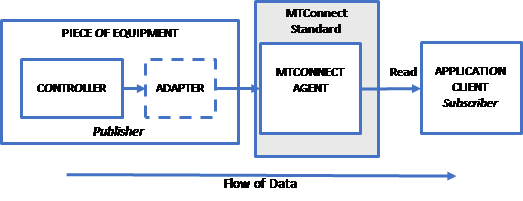
\includegraphics[width=1.0\textwidth]{figures/mtconnect-architecture-model.png}
  \caption{MTConnect Architecture Model}
  \label{fig:mtconnect-architecture-model}
\end{figure}

\FloatBarrier

\begin{note}
Note: In each implementation of a communication system based on the MTConnect Standard, there \MUST be a schema defined that encodes the rules and terminology defined for each of the \glspl{semantic data model}.  These schemas \MAY be used by client software applications to validate the content and structure of the \glspl{response document} published by an \gls{agent}.

\end{note}

\subsection{Agent}

An \gls{agent} is the centerpiece of an MTConnect implementation.  It provides two primary functions:

\begin{itemize}

\item Organizes and manages individual pieces of information published by one or more pieces of equipment.

\item Publishes that information in the form of a \gls{response document} to client software applications.

\end{itemize}

The MTConnect Standard addresses the behavior of an \gls{agent} and the structure and meaning of the data published by an \gls{agent}.  It is the responsibility of the implementer of an \gls{agent} to determine the means by which the behavior is achieved for a specific \gls{agent}.

An \gls{agent} is software that may be installed as part of a piece of equipment or it may be installed separately.  When installed separately, an \gls{agent} may receive information from one or more pieces of equipment.

Some pieces of equipment may be able to communicate directly to an \gls{agent}.  Other pieces of equipment may require an \gls{adapter} to transform the information provided by the equipment into a form that can be sent to an \gls{agent}.  In either case, the method of transmitting information from the piece of equipment to an \gls{agent} is implementation dependent and is not addressed as part of the MTConnect Standard.

One function of an \gls{agent} is to store information that it receives from a piece of equipment in an organized manner.  A second function of an \gls{agent} is to receive \glspl{request} for information from one or many client software applications and then respond to those \glspl{request} by publishing a \gls{response document} that contains the requested information.

There are three types of information stored by an \gls{agent} that \MAY be published in a \gls{response document}.  These are:

\begin{itemize}

\item \gls{equipment metadata} defines the \glspl{structural element} that represent the physical and logical parts and sub-parts of each piece of equipment that can publish data to the \gls{agent}, the relationships between those parts and sub-parts, and the \glspl{data entity} associated with each of those \glspl{structural element}.  This \gls{equipment metadata} is provided in an \gls{mtconnectdevices response document}. See \citetitle{MTCPart2} for more information on \gls{equipment metadata}.

\item \gls{streaming data} provides the values published by pieces of equipment for the \glspl{data entity} defined by the \gls{equipment metadata}.  \gls{streaming data} is provided in an \gls{mtconnectstreams response document}.  See \citetitle{MTCPart2} for more information on \gls{streaming data}.

\item \glspl{mtconnect asset} represent information used in a manufacturing operation that is commonly shared amongst multiple pieces of equipment and/or software applications.  \glspl{mtconnect asset} are provided in an \gls{mtconnectassets response document}.  See \citetitle{MTCPart40} for more information on \glspl{mtconnect asset}.

\end{itemize}

The exchange between an \gls{agent} and a client software application is a \gls{request} and \gls{response} information exchange mechanism.  See \sect{Request/Response Information Exchange} for details on this \gls{requestresponse} information exchange mechanism.

\subsubsection{Instance of an Agent}
\label{sec:Instance of an Agent}

As described above, an \gls{agent} collects and organizes values published by pieces of equipment.  As with any piece of software, an \gls{agent} may be periodically restarted.  When an \gls{agent} restarts, it \MUST indicate to client software applications whether the information available in the \gls{buffer} represents a completely new set of data or if the \gls{buffer} includes data that had been collected prior to the restart of the \gls{agent}.

Any time an \gls{agent} is restarted and begins to collect a completely new set of \gls{streaming data}, that set of data is referred to as an \gls{instance} of the \gls{agent}.  The \gls{agent} \MUST maintain a piece of information called \gls{instanceid} that represents the specific \gls{instance} of the \gls{agent}.

\gls{instanceid} is represented by a 64-bit integer.  The \gls{instanceid} \MAY be implemented using any mechanism that will guarantee that the value for \gls{instanceid} will be unique each time the \gls{agent} begins collecting a new set of data.

When an \gls{agent} is restarted and it provides a method to recover all, or some portion, of the data that was stored in the \gls{buffer} before it stopped operating, the \gls{agent} \MUST use the same \gls{instanceid} that was defined prior to the restart. 

\subsubsection{Storage of Equipment Metadata for a Piece of Equipment}

An \gls{agent} \MUST be capable of publishing \gls{equipment metadata} for each piece of equipment that publishes information through the \gls{agent}.  \gls{equipment metadata} is typically a static file defining the \glspl{structural element} associated with each piece of equipment reporting information through the \gls{agent} and the \glspl{data entity} that can be associated with each of these \glspl{structural element}.  See details on \glspl{structural element} and \glspl{data entity} in \citetitle{MTCPart2}.

The MTConnect Standard does not define the mechanism to be used by an \gls{agent} to acquire, maintain, or store the \gls{equipment metadata}.  This mechanism \MUST be defined as part of the implementation of a specific \gls{agent}.

\subsubsection{Storage of Streaming Data}

\gls{streaming data} that is published from a piece(s) of equipment to an \gls{agent} is stored by the \gls{agent} based upon the sequence upon which each piece of data is received.  As described below, the order in which data is stored by the \gls{agent} is one of the factors that determines the data that may be included in a specific \gls{mtconnectstreams response document}. 

\paragraph{Management of Streaming Data Storage}\mbox{}
\label{sec:Management of Streaming Data Storage}

An \gls{agent} stores a fixed amount of data.  The amount of data stored by an \gls{agent} is dependent upon the implementation of a specific \gls{agent}.  The examples below demonstrate how discrete pieces of data received from pieces of equipment are stored.

The method for storing \gls{streaming data} in an \gls{agent} can be thought of as a tube that can hold a finite set of balls.  Each ball represents the occurrence of a \gls{data entity} published by a piece of equipment.  This data is pushed in one end of the tube until there is no more room for additional balls.  At that point, any new data inserted will push the oldest data out the back of the tube.  The data in the tube will continue to shift in this manner as new data is received.

This tube is referred to as a \gls{buffer} in an \gls{agent}.

\begin{figure}[ht]
  \centering
  
\includegraphics[width=1.0\textwidth]{figures/data-storage-in-buffer.png}
  \caption{Data Storage in Buffer}
  \label{fig:data-storage-in-buffer}
\end{figure}

\FloatBarrier

In \fig{first-in-first-out-buffer-management}, the maximum number of \glspl{data entity} that can be stored in the \gls{buffer} of the \gls{agent} is 8.  The maximum number of \glspl{data entity} that can be stored in the \gls{buffer} is represented by a value called \gls{buffersize}.  This example illustrates that when the \gls{buffer} fills up, the oldest piece of data falls out the other end.

\begin{figure}[ht]
  \centering
  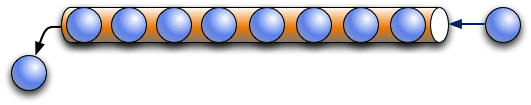
\includegraphics[width=1.0\textwidth]{figures/first-in-first-out-buffer-management.png}
  \caption{First In First Out Buffer Management}
  \label{fig:first-in-first-out-buffer-management}
\end{figure}

\FloatBarrier

This process constrains the memory storage requirements for an \gls{agent} to a fixed maximum size since the MTConnect Standard only requires an \gls{agent} to store a finite number of pieces of data.

As an implementation guideline, the \gls{buffer} \SHOULD be sized large enough to provide storage for a reasonable amount of information received from all pieces of equipment that are publishing information to that \gls{agent}.  The implementer should also consider the impact of a temporary loss of communications between a client software application and an \gls{agent} when determining the size for the \gls{buffer}.  A larger \gls{buffer} will allow a client software application more time to reconnect to an \gls{agent} without losing data.

\paragraph{Sequence Numbers}\mbox{}

In an \gls{agent}, each occurrence of a \gls{data entity} in the \gls{buffer} will be assigned a monotonically increasing \gls{sequence number} as it is inserted into the \gls{buffer}.  The \gls{sequence number} is a 64-bit integer and the values assigned as \glspl{sequence number} will never wrap around or be exhausted; at least within the next 100,000 years based on the size of a 64-bit number.

\gls{sequence number} is the primary key identifier used to manage and locate a specific piece of data in an \gls{agent}.  The \gls{sequence number} associated with each \gls{data entity} reported by an \gls{agent} is identified with an attribute called \gls{sequence}.

The \gls{sequence number} for each piece of data \MUST be unique for an instance of an \gls{agent} (see \sect{Instance of an Agent} for information on \glspl{instance} of an \gls{agent}).  If data is received from more than one piece of equipment, the \glspl{sequence number} are based on the order in which the data is received regardless of which piece of equipment produced that data.  The \gls{sequence number} \MUST be a monotonically increasing number that spans all pieces of equipment publishing data to an \gls{agent}.  This allows for multiple pieces of equipment to publish data through a single \gls{agent} with no \gls{sequence number} collisions and unnecessary protocol complexity.

The \gls{sequence number} \MUST be reset to one (1) each time an \gls{agent} is restarted and begins to collect a fresh set of data; i.e., each time \gls{instanceid} is changed.

\fig{instanceid-and-sequence} demonstrates the relationship between \gls{instanceid} and sequence when an \gls{agent} stops and restarts and begins collecting a new set of data.  In this case, the \gls{instanceid} is changed to a new value and value for \gls{sequence} resets to one (1):

\begin{figure}[ht]
  \centering
  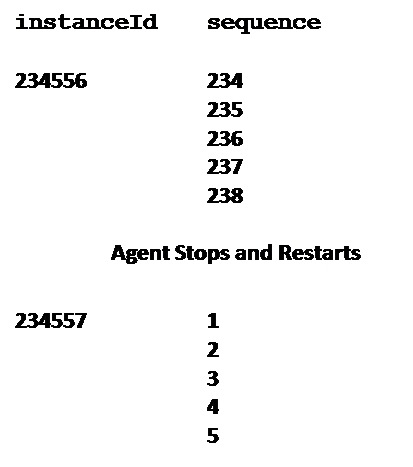
\includegraphics[width=0.5\textwidth]{figures/instanceid-and-sequence.png}
  \caption{instanceId and sequence}
  \label{fig:instanceid-and-sequence}
\end{figure}

\FloatBarrier


\fig{identifying-the-range-of-data-with-firstsequence-and-lastsequence} also shows two additional pieces of information defined for an \gls{agent}:

\begin{itemize}
\item \gls{firstsequence} -- the oldest piece of data contained in the \gls{buffer}; i.e., the next piece of data to be moved out of the \gls{buffer}

\item \gls{lastsequence} -- the newest data added to the \gls{buffer}
\end{itemize}

\gls{firstsequence} and \gls{lastsequence} provide guidance to a software application identifying the range of data available that may be requested from an \gls{agent}. 

\begin{figure}[ht]
  \centering
  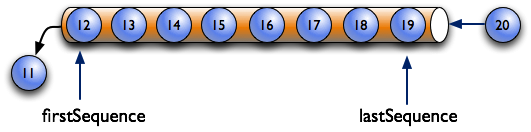
\includegraphics[width=1.0\textwidth]{figures/identifying-the-range-of-data-with-firstsequence-and-lastsequence.png}
  \caption{Indentifying the range of data with firstSequence and lastSequence}
  \label{fig:identifying-the-range-of-data-with-firstsequence-and-lastsequence}
\end{figure}

\FloatBarrier

When a client software application requests data from an \gls{agent}, it can specify both the \gls{sequence number} of the first piece of data (\gls{from query}) that \MUST be included in the \gls{response document} and the total number (\gls{count model}) of pieces of data that \SHOULD be included in that document.

In \fig{identifying-the-range-of-data-with-from-and-count}, the request specifies that the data to be returned starts at \gls{sequence number} 15 (\gls{from query}) and includes a total of three items (\gls{count model}).  

\begin{figure}[ht]
  \centering
  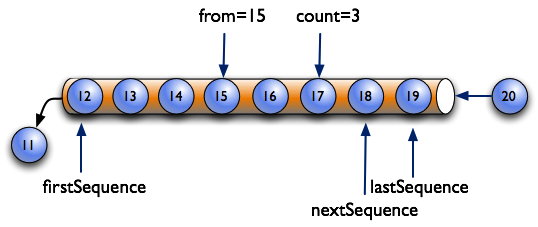
\includegraphics[width=1.0\textwidth]{figures/identifying-the-range-of-data-with-from-and-count.png}
  \caption{Identifying the range of data with from and count}
  \label{fig:identifying-the-range-of-data-with-from-and-count}
\end{figure}

\FloatBarrier


Once a \gls{response} to a \gls{request} has been completed, the value of \gls{nextsequence} will be established.  \gls{nextsequence} is the \gls{sequence number} of the next piece of data available in the \gls{buffer}.  In the example in \fig{identifying-the-range-of-data-with-from-and-count}, the next \gls{sequence number} (\gls{nextsequence}) will be 18.

As shown in \fig{identifying-the-range-of-data-with-nextsequence-and-lastsequence}, the combination of \gls{from query} and \gls{count model} defined by the \gls{request} indicates a \gls{sequence number} for data that is beyond that which is currently in the \gls{buffer}.  In this case, \gls{nextsequence} is set to a value of \gls{lastsequence} + 1.  

\begin{figure}[ht]
  \centering
  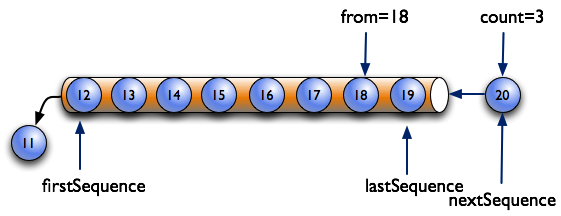
\includegraphics[width=1.0\textwidth]{figures/identifying-the-range-of-data-with-nextsequence-and-lastsequence.png}
  \caption{Indentifying the range of data with nextSequence and lastSequence}
  \label{fig:identifying-the-range-of-data-with-nextsequence-and-lastsequence}
\end{figure}

\FloatBarrier

\paragraph{Buffer Data Structure}\mbox{}

The information in the \gls{buffer} of an \gls{agent} can be thought of as a four-column table of data.  Each column in the table represents:

\begin{itemize}
\item The first column is the \gls{sequence number} associated with each \gls{data entity} - \gls{sequence}.

\item The second column is the time that the data was published by a piece of equipment.  This time is defined as the \gls{timestamp} associated with that \gls{data entity}.  See \sect{Time Stamp} for details on \gls{timestamp}.

\item The third column, \gls{dataitemid}, refers to the identity of \glspl{data entity} as they will appear in the \gls{mtconnectstreams response document}.  See \textit{Section 5} of \citetitle{MTCPart3} for details on \gls{dataitemid} for a \gls{data entity} and how that identify relates to the \gls{id} attribute of the corresponding \gls{data entity} in the \glspl{device information model}.

\item The fourth column is the value associated with each \gls{data entity}.
\end{itemize}

\fig{data-storage-concept} is an example demonstrating the concept of how data may be stored in an \gls{agent}:

\begin{figure}[ht]
  \centering
  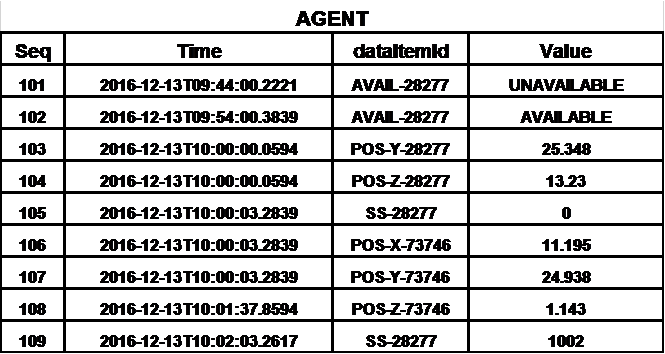
\includegraphics[width=1.0\textwidth]{figures/data-storage-concept.png}
  \caption{Data Storage Concept}
  \label{fig:data-storage-concept}
\end{figure}

\FloatBarrier


The storage mechanism for the data, the internal representation of the data, and the implementation of the \gls{agent} itself is not part of the MTConnect Standard.  The implementer can choose both the amount of data to be stored in the \gls{agent} and the mechanism for how the data is stored.  The only requirement is that an \gls{agent} publish the \glspl{response document} in the required format.  

\paragraph{Time Stamp}\mbox{}
\label{sec:Time Stamp}

Each piece of equipment that publishes information to an \gls{agent} \SHOULD provide a time stamp indicating when each piece of information was measured or determined.  If no time stamp is provided, the \gls{agent} \MUST provide a time stamp for the information based upon when that information was received at the \gls{agent}.

The \gls{timestamp} associated with each piece of information is reported by an \gls{agent} as \gls{timestamp}.  \gls{timestamp} \MUST be reported in UTC (Coordinated Universal Time) format; e.g., "2010-04-01T21:22:43Z".

\begin{note}
Note:  Z refers to UTC/GMT time, not local time.

\end{note}

Client software applications should use the value of \gls{timestamp} reported for each piece of information as the means for ordering when pieces of information were generated as opposed to using \gls{sequence} for this purpose.

\begin{note}
Note: It is assumed that \gls{timestamp} provides the best available estimate of the time that the value(s) for the published information was measured or determined.

\end{note}

If two pieces of information are measured or determined at the exact same time, they \MUST be reported with the same value for \gls{timestamp}.  Likewise, all information that is recorded in the \gls{buffer} with the same value for \gls{timestamp} should be interpreted as having been recorded at the same point in time; even if that data was published by more than one piece of equipment. 

\paragraph{Recording Occurrences of Streaming Data}\mbox{}

An \gls{agent} \MUST record data in the \gls{buffer} each time the value for that specific piece of data changes.  If a piece of equipment publishes multiple occurrences of a piece of data with the same value, the \gls{agent} \MUSTNOT record multiple occurrence for that \gls{data entity}.

\begin{note}
Note:	There is one exception to this rule.  Some \glspl{data entity} may be defined with a \gls{representation} attribute value of \gls{discrete representation} (See \textit{Section 7.2.2.12} of \citetitle{MTCPart2} for details on \gls{representation}.)  In this case, each occurrence of the data represents a new and unique piece of information.  The \gls{agent} \MUST then record each occurrence of the \gls{data entity} that is published by a piece of equipment.

\end{note}

The value for each piece of information reported by an \gls{agent} must be considered by a client software application to be valid until such a time that another occurrence of that piece of information is published by the \gls{agent}.

\paragraph{Maintaining Last Value for Data Entities}\mbox{}

An \gls{agent} \MUST retain a copy of the last available value associated with each \gls{data entity} known to the \gls{agent}; even if an occurrence of that \gls{data entity} is no longer in the \gls{buffer}.  This function allows an \gls{agent} to provide a software application a view of the last known value for each \gls{data entity} associated with a piece of equipment.

The \gls{agent} \MUST also retain a copy of the last value associated with each \gls{data entity} that has flowed out of the \gls{buffer}.  This function allows an \gls{agent} to provide a software application a view of the last known value for each \gls{data entity} associated with a \gls{current request} with an \gls{at query} parameter in the \gls{query http request} portion of its \gls{http request line} (See \sect{Current Request Implemented Using HTTP} for details on \gls{current request}).

\newpage

\paragraph{Unavailability of Data}\mbox{}

An \gls{agent} \MUST maintain a list of \glspl{data entity} that \MAY be published by each piece of equipment providing information to the \gls{agent}.   This list of \glspl{data entity} is derived from the \gls{equipment metadata} stored in the \gls{agent} for each piece of equipment.

Each time an \gls{agent} is restarted, the \gls{agent} \MUST place an occurrence of every \gls{data entity} in the \gls{buffer}.  The value reported for each of these \glspl{data entity} \MUST be set to \gls{unavailable value} and the \gls{timestamp} for each \MUST be set to the time that the last piece of data was collected by the \gls{agent} prior to the restart.

If at any time an \gls{agent} loses communications with a piece of equipment, or the \gls{agent} is unable to determine a valid value for all, or any portion, of the \glspl{data entity} published by a piece of equipment, the \gls{agent} \MUST place an occurrence of each of these \glspl{data entity} in the \gls{buffer} with its value set to \gls{unavailable value}.  This signifies that the value is currently indeterminate and no assumptions of a valid value for the data is possible.

Since an \gls{agent} may receive information from multiple pieces of equipment, it \MUST consider the validity of the data from each of these pieces of equipment independently.

There is one exception to the rules above.  Any \gls{data entity} that is constrained to a constant data value \MUST be reported with the constant value and the \gls{agent} \MUSTNOT set the value of that \gls{data entity} to \gls{unavailable value}.

\begin{note}
Note:	The schema for the \glspl{device information model} (defined in \citetitle{MTCPart2}) defines how the value reported for an individual piece of data may be constrained to one or more specific values.

\end{note}

\paragraph{Persistence and Recovery}\mbox{}

The implementer of an \gls{agent} must decide on a strategy regarding the storage of \gls{streaming data} in the \gls{buffer} of the \gls{agent}.

In the simplest form, an \gls{agent} can hold the \gls{buffer} information in volatile memory where no data is persisted when the \gls{agent} is stopped.  In this case, the \gls{agent} \MUST update the value for \gls{instanceid} when the \gls{agent} restarts to indicate that the \gls{agent} has begun to collect a new set of data.

If the implementation of an \gls{agent} provides a method of persisting and restoring all or a portion of the information in the \gls{buffer} of the \gls{agent} (\glspl{sequence number}, \glspl{time stamp}, identify, and values), the \gls{agent} \MUSTNOT change the value of the \gls{instanceid} when the \gls{agent} restarts.  This will indicate to a client software application that it does not need to reset the value for \gls{nextsequence} when it requests the next set of data from the \gls{agent}.

When an implementer chooses to provide a method to persist the information in an \gls{agent}, they may choose to store as much data as is practical in a recoverable storage system.  Such a method may also include the ability to store historical information that has previously been pushed out of the \gls{buffer}.

\paragraph{Heartbeat}\mbox{}

An \gls{agent} \MUST provide a function that indicates to a client application that the HTTP connection is still viable during times when there is no new data available to report in a \gls{response document}.  This function is defined as \gls{heartbeat}.

\gls{heartbeat} represents the amount of time after a \gls{response document} has been published until a new \gls{response document} \MUST be published, even when no new data is available.

See \sect{Query Portion of the HTTP Request Line for a Sample Request} for more details on configuring the \gls{heartbeat} function.

\paragraph{Data Sets}\mbox{}
\label{sec:Data Sets}

See \citetitle{MTCPart3} \textit{Section Part 3: DataItem with representation of DATA\textunderscore SET} for management of \glspl{data set}.


\subsubsection{Storage of Documents for MTConnect Assets}

An \gls{agent} also stores information associated with \glspl{mtconnect asset}.

When a piece of equipment publishes a document that represents information associated with an \gls{mtconnect asset}, an \gls{agent} stores that document in a \gls{buffer}.  This \gls{buffer} is called the \glspl{asset buffer}.  The document is called an \gls{asset document}.

The \glspl{asset buffer} \MUST be a separate \gls{buffer} from the one where the \gls{streaming data} is stored.

The \gls{asset document} that is published by the piece of equipment \MUST be organized based upon one of the applicable \glspl{asset information model} defined in one of the Parts 4.x of the MTConnect Standard.

An \gls{agent} will only retain a limited number of \glspl{asset document} in the \glspl{asset buffer}.  The \glspl{asset buffer} functions similar to the \gls{buffer} for \gls{streaming data}; i.e., when the \glspl{asset buffer} is full, the oldest \gls{asset document} is pushed from the \gls{buffer}.

\fig{first-in-first-out-asset-buffer-management} demonstrates the oldest \gls{asset document} being pushed from the \glspl{asset buffer} when a new \gls{asset document} is added and the \glspl{asset buffer} is full:

\begin{figure}[ht]
  \centering
  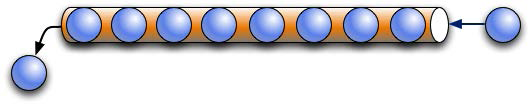
\includegraphics[width=1.0\textwidth]{figures/first-in-first-out-asset-buffer-management.png}
  \caption{First In First Out Asset Buffer Management}
  \label{fig:first-in-first-out-asset-buffer-management}
\end{figure}

\FloatBarrier

Within an \gls{agent}, the management of \glspl{asset document} behave like a key/value storage in a database.  In the case of \glspl{mtconnect asset}, the key is an identifier for an Asset (see details on \gls{assetid} in \citetitle{MTCPart40}) and the value is the \gls{asset document} that was published by the piece of equipment. 

\fig{relationship-between-assetid-and-stored-asset-documents} demonstrates the relationship between the key (\gls{assetid}) and the stored \glspl{asset document}:

\begin{figure}[ht]
  \centering
  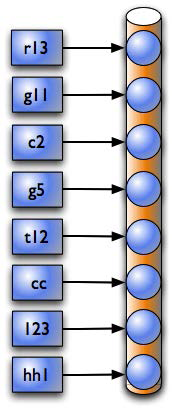
\includegraphics[width=0.3\textwidth]{figures/relationship-between-assetid-and-stored-asset-documents.png}
  \caption{Relationship between assetId and stored Asset documents}
  \label{fig:relationship-between-assetid-and-stored-asset-documents}
\end{figure}

\FloatBarrier

\begin{note}
Note:  The key (\gls{assetid}) is independent of the order of the \glspl{asset document} stored in the \glspl{asset buffer}.

\end{note}

When an \gls{agent} receives a new \gls{asset document} representing an \gls{mtconnect asset}, it must determine whether this document represents an \gls{mtconnect asset} that is not currently represented in the \glspl{asset buffer} or if the document represents new information for an \gls{mtconnect asset} that is already represented in the \glspl{asset buffer}.  When a new \gls{asset document} is received, one of the following \MUST occur:

\begin{itemize}

\item If the \gls{asset document} represents an \gls{mtconnect asset} that is not currently represented in the \glspl{asset buffer}, the \gls{agent} \MUST add the new document to the front of the \glspl{asset buffer}.  If the \glspl{asset buffer} is full, the oldest \gls{asset document} will be removed from the \glspl{asset buffer}.

\item If the \gls{asset document} represents an \gls{mtconnect asset} that is already represented in the \glspl{asset buffer}, the \gls{agent} \MUST remove the existing \gls{asset document} representing that \gls{mtconnect asset} from the \glspl{asset buffer} and add the new \gls{asset document} to the front of the \glspl{asset buffer}.  

\end{itemize}

The MTConnect Standard does not specify the maximum number of \glspl{asset document} that may be stored in the \glspl{asset buffer}; that limit is determined by the implementation of a specific \gls{agent}.  The number of \glspl{asset document} that may be stored in an \gls{agent} is defined by the value for \gls{assetbuffersize} (See \sect{Document Header} for more information on \gls{assetbuffersize}.).  A value of 4,294,967,296 or $2^{32}$ can be provided for \gls{assetbuffersize} to indicate unlimited storage.

There is no requirement for an \gls{agent} to provide persistence for the \glspl{asset document} stored in the \glspl{asset buffer}.  If an \gls{agent} should fail, all \glspl{asset document} stored in the \glspl{asset buffer} \MAY be lost.  It is the responsibility of the implementer to determine if \glspl{asset document} stored in an \gls{agent} may be restored or if those \glspl{asset document} are retained by some other software application.

Additional details on how an \gls{agent} organizes and manages information associated with \glspl{mtconnect asset} are provided in \citetitle{MTCPart40}. 

\subsection{Response Documents}

\glspl{response document} are electronic documents generated and published by an \gls{agent} in response to a \gls{request} for data. 

The \glspl{response document} defined in the MTConnect Standard are:

\begin{itemize}

\item \gls{mtconnectdevices response document}:  An electronic document that contains the information published by an \gls{agent} describing the data that can be published by one or more piece(s) of equipment.  The structure of the \gls{mtconnectdevices response document} document is based upon the requirements defined by the \glspl{device information model}.  See \citetitle{MTCPart2} for details on this information model.

\item \gls{mtconnectstreams response document}:  An electronic document that contains the information published by an \gls{agent} that contains the data that is published by one or more piece(s) of equipment.  The structure of the \gls{mtconnectstreams response document} document is based upon the requirements defined by the \gls{streams information model}.  See \citetitle{MTCPart3} for details on this information model.

\item \gls{mtconnectassets response document}:  An electronic document that contains the information published by an \gls{agent} that \MAY include one or more \glspl{asset document}.  The structure of the \gls{mtconnectassets response document} document is based upon the requirements defined by the \glspl{asset information model}.  See \citetitle{MTCPart40} for details on this information model.

\item \gls{mtconnecterrors response document}:  An electronic document that contains the information provided by an \gls{agent} when an error has occurred when trying to respond to a \gls{request} for data.  The structure of the \gls{mtconnecterrors response document} is based upon the requirements defined by the \gls{error information model}.  See \sect{Error Information Model} of this document for details on this information model.

\end{itemize}

\glspl{response document} may be represented by any document format supported by an \gls{agent}.  No matter what document format is used to structure these documents, the requirements for representing the data and other information contained in those documents \MUST adhere to the requirements defined in the \glspl{information model} associated with each document.

\subsubsection{XML Documents}
\label{sec:XML Documents}

\gls{xml} is currently the only document format supported by the MTConnect Standard for encoding \glspl{response document}.  Other document formats may be supported in the future.   

Since \gls{xml} is the document format supported by the MTConnect Standard for encoding documents, all examples demonstrating the structure of the \glspl{response document} provided throughout the MTConnect Standard are based on \gls{xml}.  These documents will be referred to as \glspl{mtconnect xml document} or \glspl{xml document}.

\sect{XML Representation of Response Documents} defines how each document is structured as an \gls{xml document}.

\subsection{Semantic Data Models}

A \gls{semantic data model} is a software engineering method for representing data where the context and the meaning of the data is constrained and fully defined.

Each of the \glspl{semantic data model} defined by the MTConnect Standard include:

\begin{itemize}
\item The types of information that may be published by a piece of equipment,

\item The meaning of that information and units of measure, if applicable,

\item Structural information that defines how different pieces of information relate to each other, and

\item Structural information that defines how the information relates to where the information was measured or generated by the piece of equipment.
\end{itemize}

As described previously, the content of the \glspl{response document} provided by an \gls{agent} are each defined by a specific \gls{semantic data model}.  The details for the \gls{semantic data model} used to define each of the \glspl{response document} are detail as follows:

\begin{itemize}
\item \gls{mtconnectdevices response document}:  \citetitle{MTCPart2}. 

\item \gls{mtconnectstreams response document}:  \citetitle{MTCPart3}.

\item \gls{mtconnectassets response document}:  \citetitle{MTCPart40} and its sub-Parts.

\item \gls{mtconnecterrors response document}:  \citetitle{MTCPart1}, \sect{Error Information Model}.
\end{itemize}

Without semantics, a single piece of data does not convey any relevant meaning to a person or a client software application.  However, when that piece of data is paired with some semantic context, the data inherits significantly more meaning.  The data can then be more completely interpreted by a client software application without human intervention.

The MTConnect \glspl{semantic data model} allows the information published by a piece of equipment to be transmitted to client software application with a full definition of the meaning of that information and in full context defining how that information relates to the piece of equipment that measured or generated the information.

\subsection{Request/Response Information Exchange}
\label{sec:Request/Response Information Exchange}

The transfer of information between an \gls{agent} and a client software application is based on a \gls{requestresponse} information exchange approach.   A client software application requests specific information from an \gls{agent}.  An \gls{agent} responds to the \gls{request} by publishing a \gls{response document}.

In normal operation, there are four types of \glspl{mtconnect request} that can be issued by a client software application that will result in different \glspl{response} by an \gls{agent}.  These \glspl{request} are:

\begin{itemize}
\item \gls{probe request}-- A client software application requests the \gls{equipment metadata} for each piece of equipment that \MAY publish information through an \gls{agent}.  The \gls{agent} publishes a \gls{mtconnectdevices response document} that contains the requested information.  A \gls{probe request} is represented by the term \gls{probe httprequest} in a \gls{request} from a client software application.

\item \gls{current request} -- A client software application requests the current value for each of the data types that have been published from a piece(s) of equipment to an \gls{agent}.  The \gls{agent} publishes a \gls{mtconnectstreams response document} that contains the requested information.  A \gls{current request} is represented by the term \gls{current httprequest} in a \gls{request} from a client software application.

\item \gls{sample request} -- A client software application requests a series of data values from the \gls{buffer} in an \gls{agent} by specifying a range of \glspl{sequence number} representing that data.  The \gls{agent} publishes a \gls{mtconnectstreams response document} that contains the requested information.  A \gls{sample request} is represented by the term \gls{sample httprequest} in a \gls{request} from a client software application.

\item \gls{asset request} -- A client software application requests information related to \glspl{mtconnect asset} that has been published to an \gls{agent}.  The \gls{agent} publishes an \gls{mtconnectassets response document} that contains the requested information.  An \gls{asset request} is represented by the term \gls{asset httprequest} in a \gls{request} from a client software application.

\begin{note}
Note: If an \gls{agent} is unable to respond to the request for information or the request includes invalid information, the \gls{agent} will publish an \gls{mtconnecterrors response document}. See \sect{Error Information Model} for information regarding \gls{error information model}

\end{note}

\end{itemize}

The specific format for the \gls{request} for information from an \gls{agent} will depend on the \gls{protocol} implemented as part of the \gls{requestresponse} information exchange mechanism deployed in a specific implementation.  See \sect{Protocol and Messaging}, \gls{protocol} for details on implementing the \gls{requestresponse} information exchange.

Also, the specific format for the \glspl{response document} may also be implementation dependent.   See \sect{XML Representation of Response Documents} for details on the format for the \glspl{response document} encoded with \gls{xml}.

\subsection{Accessing Information from an Agent}

Each of the \glspl{request} defined for the \gls{requestresponse} information exchange requires an \gls{agent} to respond with a specific view of the information stored by the \gls{agent}.  The following describes the relationships between the information stored by an \gls{agent} and the contents of the \glspl{response document}.

\subsubsection{Accessing Equipment Metadata from an Agent}

The \gls{equipment metadata} associated with each piece of equipment that publishes information to an \gls{agent} is typically static information that is maintained by the \gls{agent}.  The MTConnect Standard does not define how the \gls{agent} captures or maintains that information.  The only requirement that the MTConnect Standard places on an \gls{agent} regarding this \gls{equipment metadata} is that the \gls{agent} properly store this information and then configure and publish a \gls{mtconnectdevices response document} in response to a \gls{probe request}.

All issues associated with the capture and maintenance of the \gls{equipment metadata} is the responsibility of the implementer of a specific \gls{agent}.

\subsubsection{Accessing Streaming Data from the Buffer of an Agent}

There are two \glspl{request} defined for the \gls{requestresponse} information exchange that require an \gls{agent} to provide different views of the information stored in the \gls{buffer} of the \gls{agent}.  These \glspl{request} are \gls{current httprequest} and \gls{sample httprequest}.

The example in \fig{example-buffer} demonstrates how an \gls{agent} interprets the information stored in the \gls{buffer} to provide the content that is published in different versions of the \gls{mtconnectstreams response document} based on the specific \gls{request} that is issued by a client software application.

In this example, an \gls{agent} with a \gls{buffer} that can hold up to eight (8) \glspl{data entity}; i.e., the value for \gls{buffersize} is 8.  This \gls{agent} is collecting information for two pieces of data -- \cfont{Pos} representing a position and \cfont{Line} representing a line of logic or commands in a control program.  

In this \gls{buffer}, the value for \gls{firstsequence} is 12 and the value for \gls{lastsequence} is 19.  There are five (5) different values for \cfont{Pos} and three (3) different values for \cfont{Line}.  

\begin{figure}[ht]
  \centering
  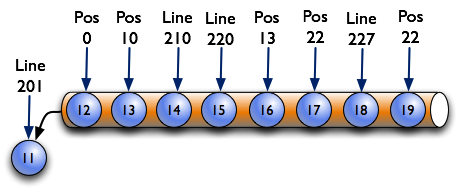
\includegraphics[width=1.0\textwidth]{figures/example-buffer.png}
  \caption{Example Buffer}
  \label{fig:example-buffer}
\end{figure}

\FloatBarrier

If an \gls{agent} receives a \gls{sample request} from a client software application, the \gls{agent} \MUST publish an \gls{mtconnectstreams response document} that contains a range of data values.  The range of values are defined by the \gls{from query} and \gls{count model} parameters that must be included as part of the \gls{sample request}.  If the value of \gls{from query} is 14 and the value of \gls{count model} is 5, the \gls{agent} \MUST publish an \gls{mtconnectstreams response document} that includes five (5) pieces of data represented by \glspl{sequence number} 14, 15, 16, 17, and 18 -- three (3) occurrences of \cfont{Line} and two (2) occurrences of \cfont{Pos}.  In this case, \gls{nextsequence} will also be returned with a value of 19.

Likewise, if the same \gls{agent} receives a \gls{current request} from a client software application, the \gls{agent} \MUST publish an \gls{mtconnectstreams response document} that contains the most current information available for each of the types of data that is being published to the \gls{agent}.  In this case, the specific data that \MUST be represented in the \gls{mtconnectstreams response document} is \cfont{Pos} with a value of 22 and a \gls{sequence number} of 19 and \cfont{Line} with a value of 227 and a \gls{sequence number} of 18.

There is also a derivation of the \gls{current request} that will cause an \gls{agent} to publish an \gls{mtconnectstreams response document} that contains a set of data relative to a specific sequence number.  The \gls{current request} \MAY include an additional parameter called \gls{at query}.  When the \gls{at query} parameter, along with an \gls{instanceid}, is included as part of a \gls{current request}, an \gls{agent} \MUST publish an \gls{mtconnectstreams response document} that contains the most current information available for each of the types of \glspl{data entity} that are being published to the \gls{agent} that occur immediately at or before the \gls{sequence number} specified with the \gls{at query} parameter.

For example, if the \gls{request} is \cfont{current?at=15}, an \gls{agent} \MUST publish a \gls{mtconnectstreams response document} that contains the most current information available for each of the \glspl{data entity} that are stored in the \gls{buffer} of the \gls{agent} with a \gls{sequence number} of 15 or lower.  In this case, the specific data that \MUST be represented in the \gls{mtconnectstreams response document} is \cfont{Pos} with a value of 10 and a \gls{sequence number} of 13 and \cfont{Line} with a value of 220 and a \gls{sequence number} of 15.

If a \gls{current httprequest} \gls{request} is received for a \gls{sequence number} of 11 or lower, an \gls{agent} \MUST return an \gls{outofrange value} \gls{mtconnecterrors response document}.  The same \gls{http error message} \MUST be given if a \gls{sequence number} is requested that is greater than the end of the \gls{buffer}.  See \sect{Error Information Model} for more information on \gls{mtconnecterrors response document}.

\subsubsection{Accessing MTConnect Assets Information from an Agent}

When an \gls{agent} receives an \gls{asset request}, the \gls{agent} \MUST publish an \gls{mtconnectassets} document that contains information regarding the \glspl{asset document} that are stored in the \gls{agent}.

See \citetitle{MTCPart40} for details on \glspl{mtconnect asset}, \glspl{asset request}, and the \gls{mtconnectassets response document}.

\section{XML Representation of Response Documents}
\label{sec:XML Representation of Response Documents}

As defined in \sect{XML Documents}, \gls{xml} is currently the only language supported by the MTConnect Standard for encoding \glspl{response document}.

\glspl{response document} must be valid and conform to the \gls{schema} defined in the \gls{semantic data model} defined for that document.  The \gls{schema} for each \gls{response document} \MUST be updated to correlate to a specific version of the MTConnect Standard.  Versions, within a \gls{major} version, of the MTConnect Standard will be defined in such a way to best maintain backwards compatibility of the \glspl{semantic data model} through all \gls{minor} revisions of the Standard.  However, new \gls{minor} versions may introduce extensions or enhancements to existing \glspl{semantic data model}.

To be valid, a \gls{response document} must be well-formed; meaning that, amongst other things, each element has the required \gls{xml} \textit{start-tag} and \textit{end-tag} and that the document does not contain any illegal characters.  The validation of the document may also include a determination that required elements and attributes are present, they only occur in the appropriate location in the document, and they appear only the correct number of times.  If the document is not well-formed, it may be rejected by a client software application.  The \gls{semantic data model} defined for each \gls{response document} also specifies the elements and \glspl{child element} that may appear in a document.  \gls{xml} elements may contain \glspl{child element}, \gls{cdata}, or both.  The \gls{semantic data model} also defines the number of times each element and \gls{child element} may appear in the document.

Each \gls{response document} encoded using \gls{xml} consists of the following primary sections:

\begin{itemize}
\item \gls{xml} Declaration

\item Root Element

\item Schema and Namespace Declaration

\item Document Header

\item Document Body
\end{itemize}

The following will provide details defining how each of the \glspl{response document} are encoded using \gls{xml}.

\begin{note}
Note: See \sect{Terminology and Conventions} for the definition of \gls{xml} related terms used in the MTConnect Standard.

\end{note}

\subsection{Fundamentals of Using XML to Encode Response Documents}

The MTConnect Standard follows industry conventions for formatting the elements and attributes included in an \gls{xml} document.  The general guidelines are as follows: 

\begin{itemize}
\item All element names \MUST be specified in Pascal case (first letter of each word is capitalized). For example: \cfont{<PowerSupply/>}.

\item The name for an attribute \MUST be Camel case; similar to Pascal case, but the first letter will be lower case.  For example: \cfont{<MyElement nativeName="bob"/>} where \cfont{MyElement} is the \gls{element name} and \gls{nativename} is an attribute.

\item All \gls{cdata} values that are defined with a limited or controlled vocabulary \MUST be in upper case with an \_ (underscore) separating words.  For example: \gls{on value}, \gls{off value}, \gls{actual subtype}, and \gls{counterclockwise value}.

\item The values provided for a date and/or a time \MUST follow the W3C ISO 8601 format with an arbitrary number of decimals representing fractions of a second.  Refer to the following specification for details on the format for dates and times:  http://www.w3.org/TR/NOTE-datetime.

The format for the value describing a date and a time will be\\ YYYY-MM-DDThh:mm:ss.ffff. An example would be: 2017-01-13T13:01.213415Z.  

\begin{note}
Note:  Z refers to UTC/GMT time, not local time.

\end{note}

The accuracy and number of decimals representing fractions of a second for a \gls{timestamp} \MUST be determined by the capabilities of the piece of equipment publishing information to an \gls{agent}.  All time values \MUST be provided in UTC (GMT).

\item \gls{xml} element names \MUST be spelled out and abbreviations are not permitted.   See the exclusion below regarding the use of the suffix \cfont{Ref}.

\item \gls{xml} attribute names \SHOULD be spelled out and abbreviations \SHOULD be avoided.  The exception to this rule is the use of \gls{id} when associated with an identifier.  See the exclusion below regarding the use of the suffix \cfont{Ref}.

\item The abbreviation \cfont{Ref} for \gls{reference} is permitted as a suffix to element names of either a \gls{structural element} or a \gls{data entity} to provide an efficient method to associate information defined in another location in a \gls{data model} without duplicating that original data or structure.  See \textit{Section 4.8} in \citetitle{MTCPart2} for more information on \gls{reference}.
\end{itemize}

\subsection{XML Declaration}

The first section of a \gls{response document} encoded with \gls{xml} \SHOULD be the \gls{xml declaration}.  The declaration is a single element.

An example of an \gls{xml declaration} would be:  

\begin{lstlisting}[firstnumber=1,escapechar=|,%
caption={Example of xml declaration}, label={lst:xml-declaration}]
<?xml version="1.0" encoding="UTF-8"?>
\end{lstlisting}

This element provides information regarding how the \gls{xml} document is encoded and the character type used for that encoding.  See the W3C website for more details on the \gls{xml} declaration. 

\subsection{Root Element}

Every \gls{response document} \MUST contain only one root element.  The MTConnect Standard defines \gls{mtconnectdevices}, \gls{mtconnectstreams}, \gls{mtconnectassets}, and \gls{mtconnecterror} as \glspl{root element}. 

The \gls{root element} specifies a specific \gls{response document} and appears at the top of the document immediately following the \gls{xml declaration}.

\subsubsection{MTConnectDevices Root Element}

\gls{mtconnectdevices} is the \gls{root element} for the \gls{mtconnectdevices response document}.  

\begin{figure}[ht]
  \centering
  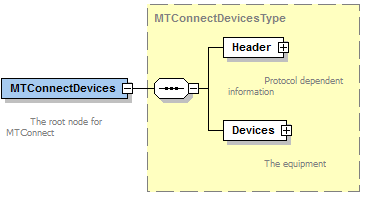
\includegraphics[width=0.7\textwidth]{figures/mtconnectdevices-structure.png}
  \caption{MTConnectDevices Structure}
  \label{fig:mtconnectdevices-structure}
\end{figure}

\FloatBarrier

\gls{mtconnectdevices} \MUST contain two \glspl{child element} - \gls{header} and \gls{devices}.  Details for \gls{header} are defined in \sect{Document Header}.  

\gls{devices} is an \gls{xml} container that represents the \gls{document body} for an \gls{mtconnectdevices response document} -- see \sect{Document Body}.  Details for the \gls{semantic data model} describing the contents for \gls{devices} are defined in \citetitle{MTCPart2}.

\gls{mtconnectdevices} also has a number of attributes.  These attributes are defined in \sect{Schema and Namespace Declaration}.

\paragraph{MTConnectDevices Elements}\mbox{}

An \gls{mtconnectdevices} element \MUST contain a \gls{header} and a \gls{devices} element.

\tabulinesep = 5pt
\begin{longtabu} to \textwidth {
    |l|X[3l]|X[0.75l]|}
\caption{Elements for MTConnectDevices} \label{table:elements-for-mtconnectdevices} \\

\hline
Element & Description & Occurrence \\
\hline
\endfirsthead

\hline
\multicolumn{3}{|c|}{Continuation of Table \ref{table:elements-for-mtconnectdevices}}\\
\hline
Element & Description & Occurrence \\
\hline
\endhead
 
\gls{header}
&
An \gls{xml} container in an \gls{mtconnect response document} that provides information from an \gls{agent} defining version information, storage capacity, and parameters associated with the data management within the \gls{agent}.
&
1 \\
\hline

\gls{devices}
&
The \gls{xml} container in an \gls{mtconnect response document} that provides the \gls{equipment metadata} for each of the pieces of equipment associated with an \gls{agent}.
&
1 \\
\hline


\end{longtabu}

\subsubsection{MTConnectStreams Root Element}

\gls{mtconnectstreams} is the \gls{root element} for the \gls{mtconnectstreams response document}.  

\begin{figure}[ht]
  \centering
  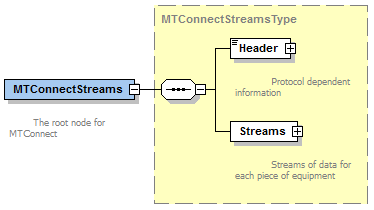
\includegraphics[width=0.7\textwidth]{figures/mtconnectstreams-structure.png}
  \caption{MTConnectStreams Structure}
  \label{fig:mtconnectstreams-structure}
\end{figure}

\FloatBarrier

\gls{mtconnectstreams} \MUST contain two \glspl{child element} - \gls{header} and \gls{streams}.  

Details for \gls{header} are defined in \sect{Document Header}.  

\gls{streams} is an \gls{xml} container that represents the \gls{document body} for a \gls{mtconnectstreams response document} -- see \sect{Document Body}.  Details for the \gls{semantic data model} describing the contents for \gls{streams} are defined in \citetitle{MTCPart3}.

\gls{mtconnectstreams} also has a number of attributes.  These attributes are defined in \sect{Schema and Namespace Declaration}.

\newpage

\paragraph{MTConnectStreams Elements}\mbox{}

An \gls{mtconnectstreams} element \MUST contain a \gls{header} and a \gls{streams} element.

\tabulinesep = 5pt
\begin{longtabu} to \textwidth {
    |l|X[3l]|X[0.75l]|}
\caption{Elements for MTConnectStreams} \label{table:elements-for-mtconnectstreams} \\

\hline
Element & Description & Occurrence \\
\hline
\endfirsthead

\hline
\multicolumn{3}{|c|}{Continuation of Table \ref{table:elements-for-mtconnectstreams}}\\
\hline
Element & Description & Occurrence \\
\hline
\endhead
 
\gls{header}
&
An \gls{xml} container in an \gls{mtconnect response document} that provides information from an \gls{agent} defining version information, storage capacity, and parameters associated with the data management within the \gls{agent}.
&
1 \\
\hline

\gls{streams}
&
The \gls{xml} container for the information published by an \gls{agent} in a \gls{mtconnectstreams response document}.
&
1 \\
\hline


\end{longtabu}

\subsubsection{MTConnectAssets Root Element}

\gls{mtconnectassets} is the \gls{root element} for the \gls{mtconnectassets response document}.  

\begin{figure}[ht]
  \centering
  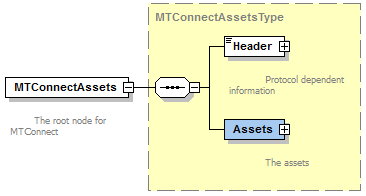
\includegraphics[width=0.7\textwidth]{figures/mtconnectassets-structure.png}
  \caption{MTConnectAssets Structure}
  \label{fig:mtconnectassets-structure}
\end{figure}

\FloatBarrier

\newpage 

\gls{mtconnectassets} \MUST contain two \glspl{child element} - \gls{header} and \gls{assets mtconnectassets}.

Details for \gls{header} are defined in \sect{Document Header}.  

\gls{assets mtconnectassets} is an \gls{xml} container that represents the \gls{document body} for an \gls{mtconnectassets response document} -- see \sect{Document Body}.  Details for the \gls{semantic data model} describing the contents for \gls{assets mtconnectassets} are defined in \citetitle{MTCPart40}.

\gls{mtconnectassets} also has a number of attributes.  These attributes are defined in \sect{Schema and Namespace Declaration}.

\paragraph{MTConnectAssets Elements}\mbox{}

An \gls{mtconnectassets} element \MUST contain a \gls{header} and an \gls{assets mtconnectassets} element.

\tabulinesep = 5pt
\begin{longtabu} to \textwidth {
    |l|X[3l]|X[0.75l]|}
\caption{Elements for MTConnectAssets} \label{table:elements-for-mtconnectassets} \\

\hline
Element & Description & Occurrence \\
\hline
\endfirsthead

\hline
\multicolumn{3}{|c|}{Continuation of Table \ref{table:elements-for-mtconnectassets}}\\
\hline
Element & Description & Occurrence \\
\hline
\endhead
 
\gls{header}
&
An \gls{xml} container in an \gls{mtconnect response document} that provides information from an \gls{agent} defining version information, storage capacity, and parameters associated with the data management within the \gls{agent}.
&
1 \\
\hline

\gls{assets mtconnectassets}
&
The \gls{xml} container in an \gls{mtconnectassets response document} that provides information for \glspl{mtconnect asset} associated with an \gls{agent}.
&
1 \\
\hline


\end{longtabu}

\subsubsection{MTConnectError Root Element}

\gls{mtconnecterror} is the \gls{root element} for the \gls{mtconnecterrors response document}.

\begin{figure}[ht]
  \centering
  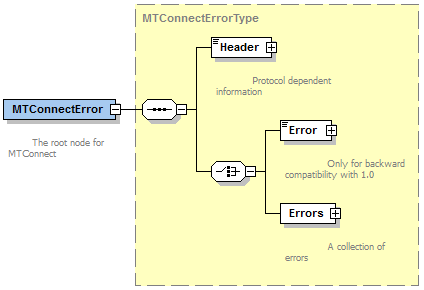
\includegraphics[width=0.7\textwidth]{figures/mtconnecterror-structure.png}
  \caption{MTConnectError Structure}
  \label{fig:mtconnecterror-structure}
\end{figure}

\FloatBarrier

\gls{mtconnecterror} \MUST contain two \glspl{child element} - \gls{header} and \gls{errors}. 

\begin{note}
Note:	When compatibility with \textit{Version 1.0.1} and earlier of the MTConnect Standard is required for an implementation, the \gls{mtconnecterrors response document} contains only a single \gls{error} \gls{data entity} and the \gls{errors} \gls{child element} \MUSTNOT appear in the document. 

\end{note}

Details for \gls{header} are defined in \sect{Document Header}.  

\gls{errors} is an \gls{xml} container that represents the \gls{document body} for an \gls{mtconnecterrors response document} -- See \sect{Document Body}.  Details for the \gls{semantic data model} describing the contents for \gls{errors} are defined in \sect{Error Information Model}.

\gls{mtconnecterror} also has a number of attributes.  These attributes are defined in \sect{Schema and Namespace Declaration}.

\paragraph{MTConnectError Elements}\mbox{}

An \gls{mtconnecterror} element \MUST contain a \gls{header} and an \gls{errors} element.

\tabulinesep = 5pt
\begin{longtabu} to \textwidth {
    |l|X[3l]|X[0.75l]|}
\caption{Elements for MTConnectError} \label{table:elements-for-mtconnecterror} \\

\hline
Element & Description & Occurrence \\
\hline
\endfirsthead

\hline
\multicolumn{3}{|c|}{Continuation of Table \ref{table:elements-for-mtconnecterror}}\\
\hline
Element & Description & Occurrence \\
\hline
\endhead
 
\gls{header}
&
An \gls{xml} container in an \gls{mtconnect response document} that provides information from an \gls{agent} defining version information, storage capacity, and parameters associated with the data management within the \gls{agent}.
&
1 \\
\hline

\gls{errors}
&
The \gls{xml} container in an \gls{mtconnecterrors response document} that provides information associated with errors encountered by an \gls{agent}.
&
1 \\
\hline


\end{longtabu}

\subsection{Schema and Namespace Declaration}
\label{sec:Schema and Namespace Declaration}

\gls{xml} provides standard methods for declaring the \gls{schema} and \gls{namespace} associated with a document encoded by \gls{xml}.  The declaration of the \gls{schema} and \gls{namespace} for MTConnect \glspl{response document} \MUST be structured as attributes in the \gls{root element} of the document.  \gls{xml} defines these attributes as pseudo-attributes since they provide additional information for the entire document and not just specifically for the \gls{root element} itself.  

\begin{note}
Note:	If a \gls{response document} contains sections that utilize different \glspl{schema} and/or \glspl{namespace}, additional pseudo-attributes should appear in the document as declared using standard conventions as defined be W3C.

\end{note}

For further information on declarations refer to \apx{Schema and Namespace Declaration Information}.

\subsection{Document Header}
\label{sec:Document Header}

The \gls{document header} is an \gls{xml} container in an \gls{mtconnect response document} that provides information from an \gls{agent} defining version information, storage capacity, and parameters associated with the data management within the \gls{agent}.  This \gls{xml} element is called \gls{header}.

\gls{header} \MUST be the first \gls{xml} element following the \gls{root element} of any \gls{response document}.  The \gls{header} \gls{xml} element \MUSTNOT contain any \glspl{child element}.  

The content of the \gls{header} element will be different for each type of \gls{response document}.

\subsubsection{Header for MTConnectDevices}

The \gls{header} element for an \gls{mtconnectdevices response document} defines information regarding the creation of the document and the data storage capability of the \gls{agent} that generated the document.  

\paragraph{XML Schema Structure for Header for MTConnectDevices}\mbox{}

The \gls{xml schema} in \fig{header-schema-diagram-for-mtconnectdevices} represents the structure of the \gls{header} \gls{xml} element that \MUST be provided for an \gls{mtconnectdevices response document}.  

\begin{figure}[ht]
  \centering
  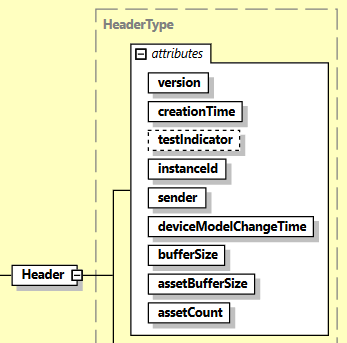
\includegraphics[width=0.6\textwidth]{figures/header-schema-diagram-for-mtconnectdevices.png}
  \caption{Header Schema Diagram for MTConnectDevices}
  \label{fig:header-schema-diagram-for-mtconnectdevices}
\end{figure}

\FloatBarrier

\paragraph{Attributes for Header for MTConnectDevices}\mbox{}

\tbl{attributes-for-header-mtconnectdevices} defines the attributes that may be used to provide additional information in the \gls{header} element for an \gls{mtconnectdevices response document}. 

\tabulinesep = 5pt
\begin{longtabu} to \textwidth {
    |l|X[3l]|X[0.75l]|}
\caption{MTConnectDevices Header} \label{table:attributes-for-header-mtconnectdevices} \\

\hline
Attribute & Description & Occurrence \\
\hline
\endfirsthead

\hline
\multicolumn{3}{|c|}{Continuation of Table \ref{table:attributes-for-header-mtconnectdevices}}\\
\hline
Attribute & Description & Occurrence \\
\hline
\endhead
 
\gls{version}
&
The \gls{major}, \gls{minor}, and \gls{revision} number of the MTConnect Standard that defines the \gls{semantic data model} that represents the content of the \gls{response document}.   It also includes the revision number of the \gls{schema} associated with that specific \gls{semantic data model}.
\newline The value reported for \gls{version} \MUST be a series of four numeric values, separated by a decimal point, representing a \gls{major}, \gls{minor}, and \gls{revision} number of the MTConnect Standard and the revision number of a specific \gls{schema}.  
\newline As an example, the value reported for \gls{version} for a \gls{response document} that was structured based on \gls{schema} revision 10 associated with Version 1.4.0 of the MTConnect Standard would be:  1.4.0.10
\newline \gls{version} is a required attribute.
&
1 \\
\hline

\gls{creationtime}
&
\gls{creationtime} represents the time that an \gls{agent} published the \gls{response document}. 
\newline \gls{creationtime} \MUST be reported in UTC (Coordinated Universal Time) format; e.g., "2010-04-01T21:22:43Z".
\newline Note:  Z refers to UTC/GMT time, not local time.
\newline \gls{creationtime} is a required attribute.
&
1 \\
\hline

\gls{testindicator}
&
A flag indicating that the \gls{agent} that published the \gls{response document} is operating in a test mode.  The contents of the \gls{response document} may not be valid and SHOULD be used for testing and simulation purposes only. 
\newline The values reported for \gls{testindicator} are:
\newline -	  \gls{true value}:  The \gls{agent} is functioning in a test mode.
\newline -	  \gls{false value}:  The \gls{agent} is not functioning in a test mode.
\newline If \gls{testindicator} is not specified, the value for \gls{testindicator} \MUST be interpreted to be \gls{false value}.
\newline \gls{testindicator} is an optional attribute.
&
0..1 \\
\hline

\gls{instanceid}
&
A number indicating a specific instantiation of the \gls{buffer} associated with the \gls{agent} that published the \gls{response document}.  
\newline The value reported for \gls{instanceid} \MUST be a unique unsigned 64-bit integer.   
\newline The value for \gls{instanceid} \MUST be changed to a different unique number each time the \gls{buffer} is cleared and a new set of data begins to be collected.
\newline \gls{instanceid} is a required attribute.
&
1 \\
\hline

\gls{sender}
&
An identification defining where the \gls{agent} that published the \gls{response document} is installed or hosted.
\newline The value reported for \gls{sender} \MUST be either an IP Address or Hostname describing where the \gls{agent} is installed or the URL of the \gls{agent}; e.g., \cfont{http://<address>[:port]/}. 
\newline Note:  The port number need not be specified if it is the default HTTP port 80.
\newline \gls{sender} is a required attribute.
&
1 \\
\hline

\gls{buffersize}
&
A value representing the maximum number of \glspl{data entity} that \MAY be retained in the \gls{agent} that published the \gls{response document} at any point in time.
\newline The value reported for \gls{buffersize} \MUST be a number representing an unsigned 32-bit integer.
\newline \gls{buffersize} is a required attribute. 
\newline Note 1:  \gls{buffersize} represents the maximum number of sequence numbers that \MAY be stored in the \gls{agent}. 
\newline Note 2: The implementer is responsible for allocating the appropriate amount of storage capacity required to accommodate the \gls{buffersize}.
&
1 \\
\hline


\gls{assetbuffersize}
&
A value representing the maximum number of \glspl{asset document} that can be stored in the \gls{agent} that published the \gls{response document}.  
\newline The value reported for \gls{assetbuffersize} \MUST be a number representing an unsigned 32-bit integer.
\newline \gls{assetbuffersize} is a required attribute.
\newline Note: The implementer is responsible for allocating the appropriate amount of storage capacity required to accommodate the \gls{assetbuffersize}.
&
1 \\
\hline

\gls{assetcount}
&
A number representing the current number of \glspl{asset document} that are currently stored in the \gls{agent} as of the \gls{creationtime} that the \gls{agent} published the \gls{response document}.  
\newline The value reported for \gls{assetcount} \MUST be a number representing an unsigned 32-bit integer and \MUSTNOT be larger than the value reported for \gls{assetbuffersize}.
\newline \gls{assetcount} is a required attribute.
&
1 \\
\hline


\gls{devicemodelchangetime}
&
\glsentrydesc{devicemodelchangetime}
&
1 \\
\hline

\end{longtabu}

\lst{header-xml-element-for-mtconnectdevices} is an example of a \gls{header} \gls{xml} element for an \gls{mtconnectdevices response document}:

\begin{lstlisting}[firstnumber=1,escapechar=|,%
caption={Example of Header XML Element for MTConnectDevices}, label={lst:header-xml-element-for-mtconnectdevices}]
<Header creationTime="2017-02-16T16:44:27Z"
  sender="MyAgent" instanceId="1268463594"
  bufferSize="131072" version="1.4.0.10"
  assetCount="54" assetBufferSize="1024"/>
\end{lstlisting}

\subsubsection{Header for MTConnectStreams}

The \gls{header} element for an \gls{mtconnectstreams response document} defines information regarding the creation of the document and additional information necessary for an application to interact and retrieve data from the \gls{agent}.

\paragraph{XML Schema Structure for Header for MTConnectStreams}\mbox{}

The \gls{xml schema} in \fig{header-schema-diagram-for-mtconnectstreams} represents the structure of the \gls{header} \gls{xml} element that \MUST be provided for an \gls{mtconnectstreams response document}.  

\begin{figure}[ht]
  \centering
  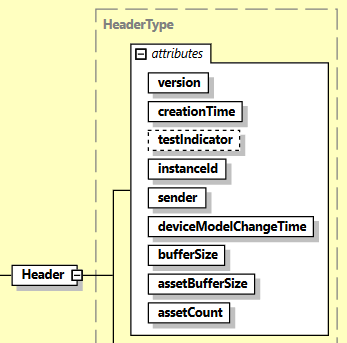
\includegraphics[width=0.6\textwidth]{figures/header-schema-diagram-for-mtconnectstreams.png}
  \caption{Header Schema Diagram for MTConnectStreams}
  \label{fig:header-schema-diagram-for-mtconnectstreams}
\end{figure}

\FloatBarrier

\paragraph{Attributes for MTConnectStreams Header}\mbox{}

\tbl{attributes-for-header-mtconnectstreams} defines the attributes that may be used to provide additional information in the \gls{header} element for an \gls{mtconnectstreams response document}.

\tabulinesep = 5pt
\begin{longtabu} to \textwidth {
    |l|X[3l]|X[0.75l]|}
\caption{MTConnectStreams Header} \label{table:attributes-for-header-mtconnectstreams} \\

\hline
Attribute & Description & Occurrence \\
\hline
\endfirsthead

\hline
\multicolumn{3}{|c|}{Continuation of Table \ref{table:attributes-for-header-mtconnectstreams}}\\
\hline
Attribute & Description & Occurrence \\
\hline
\endhead
 
\gls{version}
&
The \gls{major}, \gls{minor}, and \gls{revision} number of the MTConnect Standard that defines the \gls{semantic data model} that represents the content of the \gls{response document}.   It also includes the revision number of the \gls{schema} associated with that specific \gls{semantic data model}.
\newline The value reported for \gls{version} \MUST be a series of four numeric values, separated by a decimal point, representing a \gls{major}, \gls{minor}, and \gls{revision} number of the MTConnect Standard and the revision number of a specific \gls{schema}.  
\newline As an example, the value reported for \gls{version} for a \gls{response document} that was structured based on \gls{schema} revision 10 associated with Version 1.4.0 of the MTConnect Standard would be:  1.4.0.10
\newline \gls{version} is a required attribute.
&
1 \\
\hline

\gls{creationtime}
&
\gls{creationtime} represents the time that an \gls{agent} published the \gls{response document}. 
\newline \gls{creationtime} \MUST be reported in UTC (Coordinated Universal Time) format; e.g., "2010-04-01T21:22:43Z".
\newline Note:  Z refers to UTC/GMT time, not local time.
\newline \gls{creationtime} is a required attribute.
&
1 \\
\hline

\gls{nextsequence}
&
A number representing the \gls{sequence number} of the piece of \gls{streaming data} that is the next piece of data to be retrieved from the \gls{buffer} of the \gls{agent} that was not included in the Response Document published by the \gls{agent}.
\newline If the \gls{streaming data} included in the Response Document includes the last piece of data stored in the \gls{buffer} of the \gls{agent} at the time that the document was published, then the value reported for \gls{nextsequence} \MUST be equal to \gls{lastsequence} + 1.
\newline The value reported for \gls{nextsequence} \MUST be a number representing an unsigned 64-bit integer.
\newline \gls{nextsequence} is a required attribute.
&
1 \\
\hline

\gls{lastsequence}
&
A number representing the \gls{sequence number} assigned to the last piece of \gls{streaming data} that was added to the \gls{buffer} of the \gls{agent} immediately prior to the time that the \gls{agent} published the Response Document.   
\newline The value reported for \gls{lastsequence} \MUST be a number representing an unsigned 64-bit integer.
\newline \gls{lastsequence} is a required attribute.
&
1 \\
\hline

\gls{firstsequence}
&
A number representing the \gls{sequence number} assigned to the oldest piece of \gls{streaming data} stored in the \gls{buffer} of the \gls{agent} immediately prior to the time that the \gls{agent} published the Response Document.   
\newline The value reported for \gls{firstsequence} \MUST be a number representing an unsigned 64-bit integer.
\newline \gls{firstsequence} is a required attribute.
&
1 \\
\hline

\gls{testindicator}
&
A flag indicating that the \gls{agent} that published the \gls{response document} is operating in a test mode.  The contents of the \gls{response document} may not be valid and \SHOULD be used for testing and simulation purposes only. 
\newline The values reported for \gls{testindicator} are:
\newline -	  \gls{true value}:  The \gls{agent} is functioning in a test mode.
\newline -	  \gls{false value}:  The \gls{agent} is not functioning in a test mode.
\newline If \gls{testindicator} is not specified, the value for \gls{testindicator} \MUST be interpreted to be \gls{false value}.
\newline \gls{testindicator} is an optional attribute.
&
0..1 \\
\hline

\gls{instanceid}
&
A number indicating a specific instantiation of the \gls{buffer} associated with the \gls{agent} that published the \gls{response document}.  
\newline The value reported for \gls{instanceid} \MUST be a unique unsigned 64-bit integer.   
\newline The value for \gls{instanceid} \MUST be changed to a different unique number each time the \gls{buffer} is cleared and a new set of data begins to be collected.
\newline \gls{instanceid} is a required attribute.
&
1 \\
\hline

\gls{sender}
&
An identification defining where the \gls{agent} that published the \gls{response document} is installed or hosted.
\newline The value reported for \gls{sender} \MUST be either an IP Address or Hostname describing where the \gls{agent} is installed or the URL of the \gls{agent}; e.g., \cfont{http://<address>[:port]/}. 
\newline Note:  The port number need not be specified if it is the default HTTP port 80.
\newline \gls{sender} is a required attribute.
&
1 \\
\hline

\gls{buffersize}
&
A value representing the maximum number of \glspl{data entity} that \MAY be retained in the \gls{agent} that published the \gls{response document} at any point in time.
\newline The value reported for \gls{buffersize} \MUST be a number representing an unsigned 32-bit integer.
\newline \gls{buffersize} is a required attribute. 
\newline Note 1:  \gls{buffersize} represents the maximum number of  \glspl{sequence number} that \MAY be stored in the \gls{agent}. 
\newline Note 2: The implementer is responsible for allocating the appropriate amount of storage capacity required to accommodate the \gls{buffersize}.
&
1 \\
\hline

\gls{devicemodelchangetime}
&
\glsentrydesc{devicemodelchangetime}
&
1 \\
\hline


\end{longtabu}

\lst{header-xml-element-for-mtconnectstreams} is an example of a \gls{header} \gls{xml} element for an \gls{mtconnectstreams response document}:

\begin{lstlisting}[firstnumber=1,escapechar=|,%
caption={Example of Header XML Element for MTConnectStreams}, label={lst:header-xml-element-for-mtconnectstreams}]
<Header lastSequence="5430495" firstSequence="5299424"
  nextSequence="5430496" bufferSize="131072"
  version="1.4.0.12" instanceId="1579788747"
  sender="myagent" creationTime="2020-03-24T13:23:32Z"/>
\end{lstlisting}

\subsubsection{Header for MTConnectAssets}

The \gls{header} element for an \gls{mtconnectassets response document} defines information regarding the creation of the document and the storage of \glspl{asset document} in the \gls{agent} that generated the document.  

\paragraph{XML Schema Structure for Header for MTConnectAssets}\mbox{}

The \gls{xml schema} in \fig{header-schema-diagram-for-mtconnectassets} represents the structure of the \gls{header} \gls{xml} element that \MUST be provided for an \gls{mtconnectassets response document}.  

\begin{figure}[ht]
  \centering
  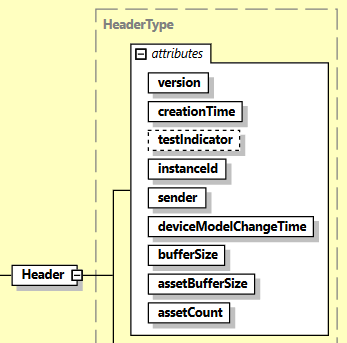
\includegraphics[width=0.6\textwidth]{figures/header-schema-diagram-for-mtconnectassets.png}
  \caption{Header Schema Diagram for MTConnectAssets}
  \label{fig:header-schema-diagram-for-mtconnectassets}
\end{figure}

\FloatBarrier

\paragraph{Attributes for Header for MTConnectAssets}\mbox{}

\tbl{attributes-for-header-mtconnectassets} defines the attributes that may be used to provide additional information in the \gls{header} element for an \gls{mtconnectassets response document}.

\tabulinesep = 5pt
\begin{longtabu} to \textwidth {
    |l|X[3l]|X[0.75l]|}
\caption{MTConnectAssets Header} \label{table:attributes-for-header-mtconnectassets} \\

\hline
Attribute & Description & Occurrence \\
\hline
\endfirsthead

\hline
\multicolumn{3}{|c|}{Continuation of Table \ref{table:attributes-for-header-mtconnectassets}}\\
\hline
Attribute & Description & Occurrence \\
\hline
\endhead
 
\gls{version}
&
The \gls{major}, \gls{minor}, and \gls{revision} number of the MTConnect Standard that defines the \gls{semantic data model} that represents the content of the \gls{response document}.   It also includes the revision number of the \gls{schema} associated with that specific \gls{semantic data model}.
\newline The value reported for \gls{version} \MUST be a series of four numeric values, separated by a decimal point, representing a \gls{major}, \gls{minor}, and \gls{revision} number of the MTConnect Standard and the revision number of a specific \gls{schema}.  
\newline As an example, the value reported for \gls{version} for a \gls{response document} that was structured based on \gls{schema} revision 10 associated with Version 1.4.0 of the MTConnect Standard would be:  1.4.0.10
\newline \gls{version} is a required attribute.
&
1 \\
\hline

\gls{creationtime}
&
\gls{creationtime} represents the time that an \gls{agent} published the \gls{response document}. 
\newline \gls{creationtime} \MUST be reported in UTC (Coordinated Universal Time) format; e.g., "2010-04-01T21:22:43Z".
\newline Note:  Z refers to UTC/GMT time, not local time.
\newline \gls{creationtime} is a required attribute.
&
1 \\
\hline

\gls{testindicator}
&
A flag indicating that the \gls{agent} that published the \gls{response document} is operating in a test mode.  The contents of the \gls{response document} may not be valid and SHOULD be used for testing and simulation purposes only. 
\newline The values reported for \gls{testindicator} are:
\newline -	  \gls{true value}:  The \gls{agent} is functioning in a test mode.
\newline -	  \gls{false value}:  The \gls{agent} is not functioning in a test mode.
\newline If \gls{testindicator} is not specified, the value for \gls{testindicator} \MUST be interpreted to be \gls{false value}.
\newline \gls{testindicator} is an optional attribute.
&
0..1 \\
\hline

\gls{instanceid}
&
A number indicating a specific instantiation of the \gls{buffer} associated with the \gls{agent} that published the \gls{response document}.  
\newline The value reported for \gls{instanceid} \MUST be a unique unsigned 64-bit integer.   
\newline The value for \gls{instanceid} \MUST be changed to a different unique number each time the \gls{buffer} is cleared and a new set of data begins to be collected.
\newline \gls{instanceid} is a required attribute.
&
1 \\
\hline

\gls{sender}
&
An identification defining where the \gls{agent} that published the \gls{response document} is installed or hosted.
\newline The value reported for \gls{sender} \MUST be either an IP Address or Hostname describing where the \gls{agent} is installed or the URL of the \gls{agent}; e.g., \cfont{http://<address>[:port]/}. 
\newline Note:  The port number need not be specified if it is the default HTTP port 80.
\newline \gls{sender} is a required attribute.
&
1 \\
\hline


\gls{assetbuffersize}
&
A value representing the maximum number of \glspl{asset document} that can be stored in the \gls{agent} that published the \gls{response document}.  
\newline The value reported for \gls{assetbuffersize} \MUST be a number representing an unsigned 32-bit integer.
\newline \gls{assetbuffersize} is a required attribute.
\newline Note: The implementer is responsible for allocating the appropriate amount of storage capacity required to accommodate the \gls{assetbuffersize}.
&
1 \\
\hline

\gls{assetcount}
&
A number representing the current number of \glspl{asset document} that are currently stored in the \gls{agent} as of the \gls{creationtime} that the \gls{agent} published the \gls{response document}.  
\newline The value reported for \gls{assetcount} \MUST be a number representing an unsigned 32-bit integer and \MUSTNOT be larger than the value reported for \gls{assetbuffersize}.
\newline \gls{assetcount} is a required attribute.
&
1 \\
\hline

\gls{devicemodelchangetime}
&
\glsentrydesc{devicemodelchangetime}
&
1 \\
\hline


\end{longtabu}

\lst{header-xml-element-for-mtconnectassets} is an example of a \gls{header} \gls{xml} element for an \gls{mtconnectassets response document}:

\begin{lstlisting}[firstnumber=1,escapechar=|,%
caption={Example of Header XML Element for MTConnectAssets}, label={lst:header-xml-element-for-mtconnectassets}]
<Header creationTime="2017-02-16T16:44:27Z"
  sender="MyAgent" instanceId="1268463594"
  version="1.4.0.10" assetCount="54"
  assetBufferSize="1024"/>
\end{lstlisting}

\subsubsection{Header for MTConnectError}
\label{sec:Header for MTConnectError}

The \gls{header} element for an \gls{mtconnecterrors response document} defines information regarding the creation of the document and the data storage capability of the \gls{agent} that generated the document.  

\paragraph{XML Schema Structure for Header for MTConnectError}\mbox{}

The \gls{xml schema} in \fig{header-schema-diagram-for-mtconnecterror} represents the structure of the \gls{header} \gls{xml} element that \MUST be provided for an \gls{mtconnecterrors response document}.  

\begin{figure}[ht]
  \centering
  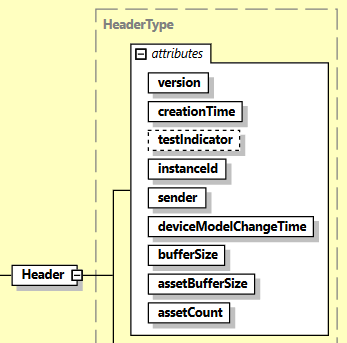
\includegraphics[width=0.6\textwidth]{figures/header-schema-diagram-for-mtconnecterror.png}
  \caption{Header Schema Diagram for MTConnectError}
  \label{fig:header-schema-diagram-for-mtconnecterror}
\end{figure}

\FloatBarrier

\paragraph{Attributes for Header for MTConnectError}\mbox{}

\tbl{attributes-for-header-mtconnecterror} defines the attributes that may be used to provide additional information in the \gls{header} element for an \gls{mtconnecterrors response document}. 

\tabulinesep = 5pt
\begin{longtabu} to \textwidth {
    |l|X[3l]|X[0.75l]|}
\caption{MTConnectError Header} \label{table:attributes-for-header-mtconnecterror} \\

\hline
Attribute & Description & Occurrence \\
\hline
\endfirsthead

\hline
\multicolumn{3}{|c|}{Continuation of Table \ref{table:attributes-for-header-mtconnecterror}}\\
\hline
Attribute & Description & Occurrence \\
\hline
\endhead
 
\gls{version}
&
The \gls{major}, \gls{minor}, and \gls{revision} number of the MTConnect Standard that defines the \gls{semantic data model} that represents the content of the \gls{response document}.   It also includes the revision number of the \gls{schema} associated with that specific \gls{semantic data model}.
\newline The value reported for \gls{version} \MUST be a series of four numeric values, separated by a decimal point, representing a \gls{major}, \gls{minor}, and \gls{revision} number of the MTConnect Standard and the revision number of a specific \gls{schema}.  
\newline As an example, the value reported for \gls{version} for a \gls{response document} that was structured based on \gls{schema} revision 10 associated with Version 1.4.0 of the MTConnect Standard would be:  1.4.0.10
\newline \gls{version} is a required attribute.
&
1 \\
\hline

\gls{creationtime}
&
\gls{creationtime} represents the time that an \gls{agent} published the \gls{response document}. 
\newline \gls{creationtime} \MUST be reported in UTC (Coordinated Universal Time) format; e.g., "2010-04-01T21:22:43Z".
\newline Note:  Z refers to UTC/GMT time, not local time.
\newline \gls{creationtime} is a required attribute.
&
1 \\
\hline

\gls{testindicator}
&
A flag indicating that the \gls{agent} that published the \gls{response document} is operating in a test mode.  The contents of the \gls{response document} may not be valid and SHOULD be used for testing and simulation purposes only. 
\newline The values reported for \gls{testindicator} are:
\newline -	  \gls{true value}:  The \gls{agent} is functioning in a test mode.
\newline -	  \gls{false value}:  The \gls{agent} is not functioning in a test mode.
\newline If \gls{testindicator} is not specified, the value for \gls{testindicator} \MUST be interpreted to be \gls{false value}.
\newline \gls{testindicator} is an optional attribute.
&
0..1 \\
\hline

\gls{instanceid}
&
A number indicating a specific instantiation of the \gls{buffer} associated with the \gls{agent} that published the \gls{response document}.  
\newline The value reported for \gls{instanceid} \MUST be a unique unsigned 64-bit integer.   
\newline The value for \gls{instanceid} \MUST be changed to a different unique number each time the \gls{buffer} is cleared and a new set of data begins to be collected.
\newline \gls{instanceid} is a required attribute.
&
1 \\
\hline

\gls{sender}
&
An identification defining where the \gls{agent} that published the \gls{response document} is installed or hosted.
\newline The value reported for \gls{sender} \MUST be either an IP Address or Hostname describing where the \gls{agent} is installed or the URL of the \gls{agent}; e.g., \cfont{http://<address>[:port]/}. 
\newline Note:  The port number need not be specified if it is the default HTTP port 80.
\newline \gls{sender} is a required attribute.
&
1 \\
\hline

\gls{buffersize}
&
A value representing the maximum number of \glspl{data entity} that \MAY be retained in the \gls{agent} that published the \gls{response document} at any point in time.
\newline The value reported for \gls{buffersize} \MUST be a number representing an unsigned 32-bit integer.
\newline \gls{buffersize} is a required attribute. 
\newline Note 1:  \gls{buffersize} represents the maximum number of sequence numbers that \MAY be stored in the \gls{agent}. 
\newline Note 2: The implementer is responsible for allocating the appropriate amount of storage capacity required to accommodate the \gls{buffersize}.
&
1 \\
\hline

\gls{devicemodelchangetime}
&
\glsentrydesc{devicemodelchangetime}
&
1 \\
\hline


\end{longtabu}

\lst{header-xml-element-for-mtconnecterror} is an example of a \gls{header} \gls{xml} element for an \gls{mtconnecterrors response document}:

\begin{lstlisting}[firstnumber=1,escapechar=|,%
caption={Example of Header XML Element for MTConnectError}, label={lst:header-xml-element-for-mtconnecterror}]
<Header creationTime="2017-02-16T16:44:27Z" 
  sender="MyAgent" instanceId="1268463594"
  bufferSize="131072" version="1.4.0.10"/>
\end{lstlisting}

\subsection{Document Body}
\label{sec:Document Body}

The \gls{document body} contains the information that is published by an \gls{agent} in response to a \gls{request} from a client software application.  Each \gls{response document} has a different \gls{xml} element that represents the \gls{document body}.

The structure of the content of the \gls{xml} element representing the \gls{document body} is defined by the \glspl{semantic data model} defined for each \gls{response document}.

\tbl{responsedocument-documentbody-semanticdatamodel} defines the relationship between each of the \glspl{response document}, the \gls{xml} element that represents the \gls{document body} for each document, and the \gls{semantic data model} that defines the structure for the content of each of the \glspl{response document}:

\tabulinesep = 5pt
\begin{longtabu} to \textwidth {
    |l|X[2l]|X[3l]|}
\caption{Relationship between Response Document and Semantic Data Model} \label{table:responsedocument-documentbody-semanticdatamodel} \\

\hline
Response Document & XML Element for Document Body & Semantic Data Model \\
\hline
\endfirsthead

\hline
\multicolumn{3}{|c|}{Continuation of Table \ref{table:responsedocument-documentbody-semanticdatamodel}}\\
\hline
Response Document & XML Element for Document Body & Semantic Data Model \\
\hline
\endhead
 
\gls{mtconnectdevices response document}
&
\gls{devices}
&
\citetitle{MTCPart2} \\
\hline

\gls{mtconnectstreams response document}
&
\gls{streams}
&
\citetitle{MTCPart3} \\
\hline

\gls{mtconnectassets response document}
&
\gls{assets mtconnectassets}
&
\citetitle{MTCPart40} \\
\hline

\gls{mtconnecterrors response document}
&
\gls{errors}
\newline Note:  \gls{errors} \MUSTNOT be used when backwards compatibility with MTConnect Standard Version 1.0.1 and earlier is required.
&
\citetitle{MTCPart1} \\
\hline

\end{longtabu}

\subsection{Extensibility}
\label{sec:Extensibility}

MTConnect is an extensible standard, which means that implementers \MAY extend the \glspl{data model} defined in the various sections of the MTConnect Standard to include information required for a specific implementation.  When these \glspl{data model} are encoded using \gls{xml}, the methods for extending these \glspl{data model} are defined by the rules established for extending any \gls{xml} schema (see the W3C website for more details on extending \gls{xml} data models).

The following are typical extensions that \MAY be considered in the MTConnect \glspl{data model}:

\begin{itemize}

\item Additional \gls{type} and \gls{subtype} values for \glspl{data entity}.

\item Additional \glspl{structural element} as containers.

\item Additional Composition elements.

\item New \gls{asset} types that are sub-typed from the abstract \gls{asset} type.

\item \glspl{child element} that may be added to specific \gls{xml} elements contained within the \glspl{mtconnect information model}.  These extended elements \MUST be identified in a separate \gls{namespace}.

\end{itemize}

When extending an MTConnect \gls{data model}, there are some basic rules restricting changes to the MTConnect \glspl{data model}.

When extending an MTConnect \gls{data model}, an implementer:

\begin{itemize}

\item \MUSTNOT add new value for category for \glspl{data entity},

\item \MUSTNOT add new \glspl{root element},

\item \SHOULDNOT add new \gls{top level} \glspl{component term}, and

\item \MUSTNOT add any new attributes or include any sub-elements to \gls{composition}.

\begin{note}
Note:  Throughout the documents additional information is provided where extensibility may be acceptable or unacceptable to maintain compliance with the MTConnect Standard.

\end{note}

\end{itemize}

When a \gls{schema} representing a \gls{data model} is extended, the \gls{schema} and \gls{namespace} declaration at the beginning of the corresponding \gls{response document} \MUST be updated to reflect the new \gls{schema} and \gls{namespace} so that a client software application can properly validate the \gls{response document}.

An \gls{xml} example of a \gls{schema} and \gls{namespace} declaration, including an extended \gls{schema} and \gls{namespace}, is shown in \lst{extended-schema-and-namespace-declaration}:

\begin{lstlisting}[firstnumber=1,escapechar=|,%
caption={Example of extended schema and namespace in declaration}, label={lst:extended-schema-and-namespace-declaration}]
<?xml version="1.0" encoding="UTF-8"?>
  <MTConnectDevices
   xmlns:xsi=http://www.w3.org/2001/XMLSchema-instance
   xmlns="urn:mtconnect.org:MTConnectDevices:1.3"
   xmlns:m="urn:mtconnect.org:MTConnectDevices:1.3"
   xmlns:x="urn:MyLocation:MyFile:MyVersion"
   xsi:schemaLocation="urn:MyLocation:MyFile:MyVersion
     /schemas/MyFileName.xsd" />
\end{lstlisting}

In this example:

\begin{itemize}

\item \cfont{xmlns:x} is added in Line 6 to identify the \gls{xml schema} instance for the extended \gls{schema}.   \glspl{element name} identified with an "\cfont{x}" prefix are associated with this specific \gls{xml schema} instance.

\begin{note}
Note: The "\cfont{x}" prefix \MAY be replaced with any prefix that the implementer chooses for identifying the extended \gls{schema} and \gls{namespace}.

\end{note}

\item \cfont{xsi:schemaLocation} is modified in Line 7 to associate the \gls{namespace} URN with the URL specifying the location of \gls{schema} file.

\item \cfont{MyLocation}, \cfont{MyFile}, \cfont{MyVersion}, and \cfont{MyFileName} in Lines 6 and 7 \MUST be replaced by the actual name, version, and location of the extended \gls{schema}.

\end{itemize}

When an extended \gls{schema} is implemented, each \gls{structural element}, \gls{data entity}, and \gls{mtconnect asset} defined in the extended \gls{schema} \MUST be identified in each respective \gls{response document} by adding a prefix to the \gls{xml} \gls{element name} associated with that \gls{structural element}, \gls{data entity}, or \gls{mtconnect asset}.  The prefix identifies the \gls{schema} and \gls{namespace} where that \gls{xml} Element is defined. 

\section{Protocol and Messaging}
\label{sec:Protocol and Messaging}

An \gls{agent} performs two \gls{major} communications tasks.  It collects information from pieces of equipment and it publishes MTConnect \glspl{response document} in response to \glspl{request} from client software applications.

The MTConnect Standard does not address the method used by an \gls{agent} to collect information from a piece of equipment.  The relationship between the \gls{agent} and a piece of equipment is implementation dependent.  The \gls{agent} may be fully integrated into the piece of equipment or the \gls{agent} may be independent of the piece of equipment.  Implementation of the relationship between a piece of equipment and an \gls{agent} is the responsibility of the supplier of the piece of equipment and/or the implementer of the \gls{agent}.

The communications mechanism between an \gls{agent} and a client software application requires the following primary components:

\begin{itemize}
\item \gls{physical connection}:  The network transmission technologies that physically interconnect an \gls{agent} and a client software application.  Examples of a \gls{physical connection} would be an Ethernet network or a wireless connection.

\item Transport Protocol:  A set of capabilities that provide the rules and procedures used to transport information between an \gls{agent} and a client software application through a \gls{physical connection}.

\item \gls{application programming interface}:  The \gls{request} and \gls{response} interactions that occur between an \gls{agent} and a client software application.

\item \gls{message term}:  The content of the information that is exchanged.  The \gls{message term} includes both the content of the MTConnect \gls{response document} and any additional information required for the client software application to interpret the \gls{response document}.

\begin{note}
Note: The \glspl{physical connection}, \glspl{transport protocol}, and \gls{application programming interface} supported by an \gls{agent} are independent of the \gls{message term} itself; i.e., the information contained in the MTConnect \glspl{response document} is not changed based on the methods used to transport those documents to a client software application.

\end{note}
\end{itemize}

An \gls{agent} \MAY support multiple methods for communicating with client software applications.  The MTConnect Standard specifies one methodology for communicating that \MUST be supported by every \gls{agent}.  This methodology is a \gls{rest}, which defines a stateless, client-server communications architecture.  This REST interface is the architectural pattern that specifies the exchange of information between an \gls{agent} and a client software application.  REST dictates that a server has no responsibility for tracking or coordinating with a client software application regarding which information or how much information the client software application may request from a server.  This removes the burden for a server to keep track of client sessions.  An \gls{agent} \MUST be implemented as a server supporting the RESTful interface. 

\section{HTTP Messaging Supported by an Agent}

This section describes the application of \gls{http messaging} applied to a REST interface that \MUST be supported by an \gls{agent} to realize the MTConnect \gls{requestresponse} information exchange functionality.

\subsection{REST Interface}

An \gls{agent} \MUST provide a REST interface that supports HTTP version 1.0 to communicate with client applications.  This interface \MUST support HTTP (RFC7230) and use URIs (RFC3986) to identify specific information requested from an \gls{agent}.  HTTP is most often implemented on top of the Transmission Control Protocol (TCP) that provides an ordered byte stream of data and the Internet Protocol (IP) that provides unified addressing and routing between computers.  However, additional interfaces to an \gls{agent} may be implemented in conjunction with any other communications technologies.

The REST interface supports an \gls{application programming interface} (API) that adheres to the architectural principles of a stateless, uniform interface to retrieve data and other information related to either pieces of equipment or \glspl{mtconnect asset}.  The API allows for access, but not modification of data stored within the \gls{agent} and is nullipotent, meaning it will not produce any side effects on the information stored in an \gls{agent} or the function of the \gls{agent} itself.

\gls{http messaging} is comprised of two basic functions -- an \gls{http request} and an \gls{http response}.  A client software application forms a \gls{request} for information from an \gls{agent} by specifying a specific set of information using an \gls{http request}.  In response, an \gls{agent} provides either an \gls{http response} or replies with an \gls{http error message} as defined below. 

\subsection{HTTP Request}

The MTConnect Standard defines that an \gls{agent} \MUST support the \cfont{HTTP GET} verb -- no other HTTP methods are required to be supported.

An \gls{http request} \MAY include three sections:

\begin{itemize}
\item an \gls{http request line}

\item \glspl{http header field}

\item an \gls{http body}
\end{itemize}

The MTConnect Standard defines that an \gls{http request} issued by a client application \SHOULD only have two sections:

\begin{itemize}
\item an \gls{http request line}

\item \glspl{http header field}
\end{itemize}

The \gls{http request line} identifies the specific information being requested by the client software application.  If an \gls{agent} receives any information in an \gls{http request} that is not specified in the MTConnect Standard, the \gls{agent} \MAY ignore it.  

The structure of an \gls{http request line} consists of the following portions:

\begin{itemize}
\item \gls{http request method}: \cfont{GET}

\item \gls{http request url}:  \cfont{http://<authority>/<path>[?<query>]}

\item \gls{http version}: \cfont{HTTP/1.0}
\end{itemize}

For the following discussion, the \gls{http request url} will only be considered since the Method will always be \cfont{GET} and the MTConnect Standard only requires \cfont{HTTP/1.0}.

\subsubsection{authority Portion of an HTTP Request Line}

The \gls{authority http request} portion consists of the DNS name or IP address associated with an \gls{agent} and an optional TCP port number [:\gls{port http request}] that the \gls{agent} is listening to for incoming \glspl{request} from client software applications.  If the port number is the default Port 80, \gls{port http request} is not required.

Example forms for \gls{authority http request} are:

\begin{itemize}
\item \cfont{http://machine/ }

\item \cfont{http://machine:5000/ }

\item \cfont{http://192.168.1.2:5000/}
\end{itemize}

\subsubsection{path Portion of an HTTP Request Line}

The \cfont{<Path>} portion of the \gls{http request line} has the follow segments:

\begin{itemize}
\item \cfont{/<name or uuid>/<request>}
\end{itemize}

In this portion of the \gls{http request line}, name or uuid designates that the information to be returned in a \gls{response document} is associated with a specific piece of equipment that has published data to the \gls{agent}.  See Part 2 - \glspl{device information model} for details on name or uuid for a piece of equipment.

\begin{note}
Note:  If \gls{name} or \gls{uuid} are not specified in the \gls{http request line}, an \gls{agent} \MUST return the information for all pieces of equipment that have published data to the \gls{agent} in the \gls{response document}.

\end{note}

In the \cfont{<Path>} portion of the \gls{http request line}, \cfont{<request>} designates one of the \glspl{request} defined in \sect{Request/Response Information Exchange}.  The value for \cfont{<request>} \MUST be \gls{probe httprequest}, \gls{current httprequest}, \gls{sample httprequest}, or \gls{asset httprequest}(s) representing the \gls{probe request}, \gls{current request}, \gls{sample request}, and \gls{asset request} respectively.  

\subsubsection{query Portion of an HTTP Request Line}

The [\cfont{?<query>}] portion of the \gls{http request line} designates an HTTP \gls{query}.  \gls{query} is a string of parameters that define filters used to refine the content of a \gls{response document} published in response to an \gls{http request}. 

\subsection{MTConnect Request/Response Information Exchange Implemented with HTTP}

An \gls{agent} \MUST support \glspl{probe request}, \glspl{current request}, \glspl{sample request}, and \glspl{asset request}.

The following sections define how the \gls{http request line} is structured to support each of these types of \glspl{request} and the information that an \gls{agent} \MUST provide in response to these \glspl{request}.

\subsubsection{Probe Request Implemented Using HTTP}

An \gls{agent} responds to a \gls{probe request} with an \gls{mtconnectdevices response document} that contains the \gls{equipment metadata} for pieces of equipment that are requested and currently represented in the \gls{agent}.  

There are two forms of the \gls{probe request}:

\begin{itemize}
\item The first form includes an \gls{http request line} that does not specify a specific path portion (\gls{name} or \gls{uuid}).  In response to this \gls{request}, the \gls{agent} returns an \gls{mtconnectdevices response document} with information for all pieces of equipment represented in the \gls{agent}.

\cfont{1.	http://<authority>/probe}

\item The second form includes an \gls{http request line} that specifies a specific path portion that defines either a \gls{name} or \gls{uuid}.  In response to this \gls{request}, the \gls{agent} returns an \gls{mtconnectdevices response document} with information for only the one piece of equipment associated with that \gls{name} or \gls{uuid}.

\cfont{1.	http://<authority>/<name or uuid>/probe}
\end{itemize}

\paragraph{Path Portion of the HTTP Request Line for a Probe Request}\mbox{}

The following segments of \gls{path query} \MUST be supported in an \gls{http request line} for a \gls{probe request}: 

\tabulinesep = 5pt
\begin{longtabu} to \textwidth {
    |l|X[3l]|}
\caption{Path of the HTTP Request Line for a Probe Request} \label{table:path-for-probe-httprequest} \\

\hline
Path Segments & Description \\
\hline
\endfirsthead

\hline
\multicolumn{2}{|c|}{Continuation of Table \ref{table:path-for-probe-httprequest}}\\
\hline
Path Segments & Description \\
\hline
\endhead

\gls{name} or \gls{uuid}
&
If present, specifies that only the \gls{equipment metadata} for the piece of equipment represented by the \gls{name} or \gls{uuid} will be published. 
\newline If not present, \gls{metadata} for all pieces of equipment associated with the \gls{agent} will be published.
\\ \hline

\cfont{<request>}
&
\gls{probe httprequest} \MUST be provided.  
\\ \hline

\end{longtabu}

\paragraph{Query Portion of the HTTP Request Line for a Probe Request}\mbox{}

The \gls{http request line} for a \gls{probe request} \SHOULDNOT contain a \gls{query http request}.  If the \gls{request} does contain a \gls{query http request}, the \gls{agent} \MUST ignore the \gls{query http request}.  

\paragraph{Response to a Probe Request}\mbox{}

The \gls{response} to a \gls{probe request} \SHOULD be an \gls{mtconnectdevices response document} for one or more pieces of equipment as designated by the \gls{path query} portion of the \gls{request}.

The \gls{response document} returned in response to a \gls{probe request} \MUST always provide the most recent information available to an \gls{agent}.

The \gls{response} \MUST also include an \gls{http status code}.   If problems are encountered by an \gls{agent} while responding to a \gls{probe request}, the \gls{agent} \MUST also publish an \gls{mtconnecterrors response document}.

\paragraph{HTTP Status Codes for a Probe Request}\mbox{}

The following \glspl{http status code} \MUST be supported as possible responses to a \gls{probe request}:

\tabulinesep = 5pt
\begin{longtabu} to \textwidth {
    |l|X[1l]|X[3l]|}
\caption{HTTP Status Codes for a Probe Request} \label{table:status-codes-for-probe-httprequest} \\

\hline
HTTP Status Code & Code Name & Description \\
\hline
\endfirsthead

\hline
\multicolumn{3}{|c|}{Continuation of Table \ref{table:status-codes-for-probe-httprequest}}\\
\hline
HTTP Status Code & Code Name & Description \\
\hline
\endhead
 
200
&
OK
&
The \gls{request} was handled successfully. \\
\hline

400
&
Bad Request
&
The \gls{request} could not be interpreted.  
\newline The \gls{agent} \MUST return a 400 \gls{http status code}.  Also, the \gls{agent} \MUST publish an \gls{mtconnecterrors response document} that identifies either \gls{invaliduri value} or \gls{invalidrequest value} as the \gls{errorcode}.
\\
\hline

404
&
Not Found
&
The \gls{request} could not be interpreted.  
\newline The \gls{agent} \MUST return a 404 \gls{http status code}.  Also, the \gls{agent} \MUST publish an \gls{mtconnecterrors response document} that identifies \gls{nodevice value} as the \gls{errorcode}.
\\
\hline

405
&
Method Not Allowed
&
A method other than \cfont{GET} was specified in the \gls{request} or the piece of equipment specified in the \gls{request} could not be found. 
\newline The \gls{agent} \MUST return a 405 \gls{http status code}.  Also, the \gls{agent} \MUST publish an \gls{mtconnecterrors response document} that identifies \gls{unsupported value} as the \gls{errorcode}. 
\\
\hline

406
&
Not Acceptable
&
The \textit{HTTP Accept Header} in the \gls{request} was not one of the supported representations. 
\newline The \gls{agent} \MUST return a 406 \gls{http status code}.  Also, the \gls{agent} \MUST publish an \gls{mtconnecterrors response document} that identifies \gls{unsupported value} as the \gls{errorcode}.
\\
\hline


431
&
Request Header Fields Too Large
&
The fields in the \gls{http request} exceed the limit of the implementation of the \gls{agent}. 
\newline The \gls{agent} \MUST return a 431 \gls{http status code}.  Also, the \gls{agent} \MUST publish an \gls{mtconnecterrors response document} that identifies \gls{invalidrequest value} as the \gls{errorcode}. 
\\
\hline


500
&
Internal Server Error
&
There was an unexpected error in the \gls{agent} while responding to a \gls{request}.  
\newline The \gls{agent} \MUST return a 500 \gls{http status code}.  Also, the \gls{agent} \MUST publish an \gls{mtconnecterrors response document} that identifies \gls{internalerror value} as the \gls{errorcode}.  
\\
\hline


\end{longtabu}

\pagebreak

\subsubsection{Current Request Implemented Using HTTP}
\label{sec:Current Request Implemented Using HTTP}

An \gls{agent} responds to a \gls{current request} with an \gls{mtconnectstreams response document} that contains the current value of \glspl{data entity} associated with each piece of \gls{streaming data} available from the \gls{agent}, subject to any filtering defined in the \gls{request}.

There are two forms of the \gls{current request}:

\begin{itemize}
\item The first form is given without a specific path portion (\gls{name} or \gls{uuid}).  In response to this \gls{request}, the \gls{agent} returns an \gls{mtconnectstreams response document} with information for all pieces of equipment represented in the \gls{buffer} of the \gls{agent}.

\cfont{1.	http://<authority>/current[?query]}

\item The second form includes a specific path portion that defines either a \gls{name} or \gls{uuid}.  In response to this \gls{request}, the \gls{agent} returns an \gls{mtconnectstreams response document} with information for only the one piece of equipment associated with the \gls{name} or \gls{uuid} defined in the \gls{request}.

\cfont{1.	http://<authority>/<name or uuid>/current[?query]}
\end{itemize}

\paragraph{Path Portion of the HTTP Request Line for a Current Request}\mbox{}

The following segments of path \MUST be supported for an \gls{http request line} for a \gls{current request}:

\tabulinesep = 5pt
\begin{longtabu} to \textwidth {
    |l|X[3l]|}
\caption{Path of the HTTP Request Line for a Current Request} \label{table:path-for-current-httprequest} \\

\hline
Path Segments & Description \\
\hline
\endfirsthead

\hline
\multicolumn{2}{|c|}{Continuation of Table \ref{table:path-for-current-httprequest}}\\
\hline
Path Segments & Description \\
\hline
\endhead

\gls{name} or \gls{uuid}
&
If present, specifies that only the \gls{equipment metadata} for the piece of equipment represented by the \gls{name} or \gls{uuid} will be published. 
\newline If not present, \gls{metadata} for all pieces of equipment associated with the \gls{agent} will be published.
\\ \hline

\cfont{<request>}
&
\gls{current httprequest} \MUST be provided. 
\\ \hline

\end{longtabu}

\paragraph{Query Portion of the HTTP Request Line for a Current Request}\mbox{}

A \gls{query} may be used to more precisely define the specific information to be included in a \gls{response document}.   Multiple parameters may be used in a \gls{query} to further refine the information to be included.   When multiple parameters are provided, each parameter is separated by an ampersand (\&) character and each parameter appears only once in the \gls{query}.  The parameters within the \gls{query} may appear in any sequence.

The following \gls{query http request} parameters \MUST be supported in an \gls{http request line} for a \gls{current request}:

\tabulinesep = 5pt
\begin{longtabu} to \textwidth {
    |l|X[3l]|}
\caption{Query Parameters of the HTTP Request Line for a Current Request} \label{table:query-parameters-for-current-httprequest} \\

\hline
Query Parameters & Description \\
\hline
\endfirsthead

\hline
\multicolumn{2}{|c|}{Continuation of Table \ref{table:query-parameters-for-current-httprequest}}\\
\hline
Query Parameters & Description \\
\hline
\endhead

\gls{path query}
&
An XPath that defines specific information or a set of information to be included in an \gls{mtconnectstreams response document}.
\newline The value for the XPath is the location of the information defined in the \glspl{device information model} that represents the \gls{structural element}(s) and/or the specific \glspl{data entity} to be included in the \gls{mtconnectstreams response document} .
\newline When a \gls{component} element is referenced by the XPath, all \gls{lower level} components and the \glspl{data entity} associated with those elements \MUST be included in the \gls{mtconnectstreams response document}. \\
\hline

\gls{at query}
&
Requests that the \glspl{mtconnect response document} \MUST include the current value for all \glspl{data entity} relative to the time that a specific \gls{sequence number} was recorded.
\newline The value associated with the \gls{at query} parameter references a specific \gls{sequence number}.  The value \MUST be an unsigned 64-bit value.
\newline The \gls{at query} parameter \MUSTNOT be used in conjunction with the \gls{interval query} parameter since this would cause an \gls{agent} to repeatedly return the same data. 
\newline If the value provided for the \gls{at query} parameter is a negative number or is not a, the \gls{request} \MUST be determined to be invalid.  The \gls{agent} \MUST return a 400 \gls{http status code}.  Also, the \gls{agent} \MUST publish an \gls{mtconnecterrors response document} that identifies an \gls{invalidrequest value} \gls{errorcode}. 
\newline If the value provided for the \gls{at query} parameter is either lower than the value of \gls{firstsequence} or greater than the value of \gls{lastsequence}, the \gls{request} \MUST be determined to be invalid.  The \gls{agent} \MUST return a 404 \gls{http status code}.  The \gls{agent} \MUST also publish an \gls{mtconnecterrors response document} that identifies an \gls{outofrange value} \gls{errorcode}. 
\newline Note:  Some information stored in the \gls{buffer} of an \gls{agent} may not be returned for a \gls{current request} with a \gls{query} containing an \gls{at query} parameter if the \gls{sequence number} associated with the most current value for that information is greater than the \gls{sequence number} specified in the \gls{query}.
\\ \hline

\gls{interval query}
&
The \gls{agent} \MUST continuously publish \glspl{response document} when the query parameters include \gls{interval query} using the value as the period between adjacent publications.
\newline The \gls{interval query} value \MUST be in milliseconds, and \MUST be a positive integer greater than zero (0).
\newline The \gls{query} \MUSTNOT specify both \gls{interval query} and \gls{at query} parameters. \\
\hline
\end{longtabu}

\paragraph{Response to a Current Request}\mbox{}

The \gls{response} to a \gls{current request} \SHOULD be an \gls{mtconnectstreams response document} for one or more pieces of equipment designated by the \gls{path query} portion of the \gls{request}.

The \gls{response} to a \gls{current request} \MUST always provide the most recent information available to an \gls{agent} or, when the \gls{at query} parameter is specified, the value of the data at the given \gls{sequence number}.

The \glspl{data entity} provided in the \gls{mtconnectstreams response document} will be limited to those specified in the combination of the \gls{path query} segment of the \gls{current request} and the value of the \gls{xpath} defined for the \gls{path query} attribute provided in the \gls{query http request} segment of that \gls{request}. 

\paragraph{HTTP Status Codes for a Current Request}\mbox{}

The following \glspl{http status code} \MUST be supported as possible responses to a \gls{current request}:

\tabulinesep = 5pt
\begin{longtabu} to \textwidth {
    |l|X[1l]|X[3l]|}
\caption{HTTP Status Codes for a Current Request} \label{table:status-codes-for-current-httprequest} \\

\hline
HTTP Status Code & Code Name & Description \\
\hline
\endfirsthead

\hline
\multicolumn{3}{|c|}{Continuation of Table \ref{table:status-codes-for-current-httprequest}}\\
\hline
HTTP Status Code & Code Name & Description \\
\hline
\endhead

200
&
OK
&
The \gls{request} was handled successfully. \\
\hline

400
&
Bad Request
&
The \gls{request} could not be interpreted.  
\newline The \gls{agent} \MUST return a 400 \gls{http status code}.  Also, the \gls{agent} \MUST publish an \gls{mtconnecterrors response document} that identifies either \gls{invaliduri value}, \gls{invalidrequest value}, or \gls{invalidxpath value} as the \gls{errorcode}.
\newline If the \gls{query http request} parameters do not contain a valid value or include an invalid parameter, the \gls{agent} \MUST return a 400 \gls{http status code}.  Also, the \gls{agent} \MUST publish an \gls{mtconnecterrors response document} that identifies \gls{queryerror value} as the \gls{errorcode}.
\\
\hline

404
&
Not Found
&
The \gls{request} could not be interpreted.  
\newline The \gls{agent} \MUST return a 404 \gls{http status code}.  Also, the \gls{agent} \MUST publish an \gls{mtconnecterrors response document} that identifies \gls{nodevice value} as the \gls{errorcode}.
\newline If the value of the \gls{at query} parameter was greater than the \gls{lastsequence} or is less than the \gls{firstsequence}, the \gls{agent} \MUST return a 404 \gls{http status code}.  Also, the \gls{agent} \MUST publish an \gls{mtconnecterrors response document} that identifies \gls{outofrange value} as the \gls{errorcode}.
\\
\hline

405
&
Method Not Allowed
&
A method other than \cfont{GET} was specified in the \gls{request} or the piece of equipment specified in the \gls{request} could not be found. 
\newline The \gls{agent} \MUST return a 405 \gls{http status code}.  Also, the \gls{agent} \MUST publish an \gls{mtconnecterrors response document} that identifies \gls{unsupported value} as the \gls{errorcode}. 
\\
\hline

406
&
Not Acceptable
&
The \textit{HTTP Accept Header} in the \gls{request} was not one of the supported representations. 
\newline The \gls{agent} \MUST return a 406 \gls{http status code}.  Also, the \gls{agent} \MUST publish an \gls{mtconnecterrors response document} that identifies \gls{unsupported value} as the \gls{errorcode}.
\\
\hline


431
&
Request Header Fields Too Large
&
The fields in the \gls{http request} exceed the limit of the implementation of the \gls{agent}. 
\newline The \gls{agent} \MUST return a 431 \gls{http status code}.  Also, the \gls{agent} \MUST publish an \gls{mtconnecterrors response document} that identifies \gls{invalidrequest value} as the \gls{errorcode}. 
\\
\hline


500
&
Internal Server Error
&
There was an unexpected error in the \gls{agent} while responding to a \gls{request}.  
\newline The \gls{agent} \MUST return a 500 \gls{http status code}.  Also, the \gls{agent} \MUST publish an \gls{mtconnecterrors response document} that identifies \gls{internalerror value} as the \gls{errorcode}.  
\\
\hline


\end{longtabu}

\subsubsection{Sample Request Implemented Using HTTP}

An \gls{agent} responds to a \gls{sample request} with an \gls{mtconnectstreams response document} that contains a set of values for \glspl{data entity} currently available for \gls{streaming data} from the \gls{agent}, subject to any filtering defined in the \gls{request}.

There are two forms to the \gls{sample request}:

\begin{itemize}
\item The first form is given without a specific \gls{path query} portion (\gls{name} or \gls{uuid}).  In response to this \gls{request}, the \gls{agent} returns an \gls{mtconnectstreams response document} with information for all pieces of equipment represented in the \gls{agent}.

\cfont{1.	http://<authority>/sample[?query]}

\item The second form includes a specific \gls{path query} portion that defines either a \gls{name} or \gls{uuid}.

In response to this \gls{request}, the \gls{agent} returns an \gls{mtconnectstreams response document} with information for only the one piece of equipment associated with the \gls{name} or \gls{uuid} defined in the \gls{request}.

\cfont{1.	http://<authority>/<name or uuid>/sample?query}
\end{itemize}

\paragraph{Path Portion of the HTTP Request Line for a Sample Request}\mbox{}

The following segments of \gls{path query} \MUST be supported in the \gls{http request line} for a \gls{sample request}:

\tabulinesep = 5pt
\begin{longtabu} to \textwidth {
    |l|X[3l]|}
\caption{Path of the HTTP Request Line for a Sample Request} \label{table:path-for-sample-httprequest} \\

\hline
Path Segments & Description \\
\hline
\endfirsthead

\hline
\multicolumn{2}{|c|}{Continuation of Table \ref{table:path-for-sample-httprequest}}\\
\hline
Path Segments & Description \\
\hline
\endhead

\gls{name} or \gls{uuid}
&
If present, specifies that only the \gls{equipment metadata} for the piece of equipment represented by the \gls{name} or \gls{uuid} will be published. 
\newline If not present, \gls{metadata} for all pieces of equipment associated with the \gls{agent} will be published.
\\ \hline

\cfont{<request>}
&
\gls{sample httprequest} \MUST be provided. 
\\ \hline

\end{longtabu}

\paragraph{Query Portion of the HTTP Request Line for a Sample Request}\mbox{}
\label{sec:Query Portion of the HTTP Request Line for a Sample Request}

A \gls{query} may be used to more precisely define the specific information to be included in a \gls{response document}.   Multiple parameters may be used in a \gls{query} to further refine the information to be included.   When multiple parameters are provided, each parameter is separated by an \& character and each parameter appears only once in the \gls{query}.  The parameters within the \gls{query} may appear in any sequence.

The following \gls{query http request} parameters \MUST be supported in an \gls{http request line} for a \gls{sample request}:

\tabulinesep = 5pt
\begin{longtabu} to \textwidth {
    |l|X[3l]|}
\caption{Query Parameters of the HTTP Request Line for a Sample Request} \label{table:query-parameters-for-sample-httprequest} \\

\hline
Query Parameters & Description \\
\hline
\endfirsthead

\hline
\multicolumn{2}{|c|}{Continuation of Table \ref{table:query-parameters-for-sample-httprequest}}\\
\hline
Query Parameters & Description \\
\hline
\endhead

\gls{path query}
&
An XPath that defines specific information or a set of information to be included in an \gls{mtconnectstreams response document}.
\newline The value for the XPath is the location of the information defined in the \glspl{device information model} that represents the \gls{structural element}(s) and/or the specific \glspl{data entity} to be included in the \gls{mtconnectstreams response document} .
\newline When a \gls{component} element is referenced by the XPath, all \gls{lower level} components and the \glspl{data entity} associated with those elements \MUST be included in the \gls{mtconnectstreams response document}. \\
\hline

\gls{from query}
&
The \gls{from query} parameter designates the \gls{sequence number} of the first \gls{observation} in the \gls{buffer} the \gls{agent} \MUST consider publishing in the \gls{response document}.
\newline The value of \gls{from query} \MUST be an unsigned 64-bit integer.
\newline If \gls{from query} is zero (0), it \MUST be set to the \gls{firstsequence}, the oldest \gls{observation} in the \gls{buffer}.
\newline If \gls{from query} and \gls{count model} parameters are not given, \gls{from query} \MUST default to the \gls{firstsequence}.
\newline If \gls{from query} is not given and \gls{count model} parameter is given, see \gls{count model} for default behavior.
\newline If the \gls{from query} parameter is less than the \gls{firstsequence} or greater than \gls{lastsequence}, the \gls{agent} \MUST return a \cfont{404} \gls{http status code} and \MUST publish an \gls{mtconnecterrors response document} with an \gls{outofrange value}  \gls{errorcode}.
\newline If the \gls{from query} parameter is not a positive numeric value, the \gls{agent} \MUST return a \cfont{400} \gls{http status code} and \MUST publish an \gls{mtconnecterrors response document} with an \gls{invalidrequest value}  \gls{errorcode}. \\
\hline

\gls{interval query}
&
The \gls{agent} \MUST continuously publish \glspl{response document} when the query parameters include \gls{interval query} using the value as the minimum period between adjacent publications.
\newline The \gls{interval query} value \MUST be in milliseconds, and \MUST be a positive integer greater than or equal to zero (0).
\newline The \gls{query} \MUSTNOT specify both \gls{interval query} and \gls{from query} parameters.
\newline If the value for the \gls{interval query} parameter is zero (0), the \gls{agent} \MUST publish  \glspl{response document} at the fastest rate possible.
\newline If the period between the publication of a \gls{response document} and reception of \glspl{observation} exceeds the \gls{interval query}, the \gls{agent} \MUST wait for a maximum of \gls{heartbeat query} milliseconds for \glspl{observation}. Upon the arrival of \glspl{observation}, the \gls{agent} \MUST immediately publish a \gls{response document}. When the period equals or exceeds the \gls{heartbeat query}, the \gls{agent} \MUST publish an empty \gls{response document}. \\
\hline

\gls{count model}
&
The \gls{count model} parameter designates the maximum number of \glspl{observation} the \gls{agent} \MUST publish in the \gls{response document}.
\newline The value of \gls{count model} \MUST be a signed integer.
\newline The \gls{count model} \MUSTNOT be zero (0).
\newline When the \gls{count model} is greater than zero (0), the \gls{from query} parameter \MUST default to the \gls{firstsequence}. The evaluation of \glspl{observation} starts at \gls{from query} and moves forward accumulating newer \glspl{observation} until the number of \glspl{observation} equals the \gls{count model} or the  \gls{observation} at \gls{lastsequence} is considered.
\newline When the \gls{count model} is less than zero (0), the \gls{from query} parameter \MUST  default to the \gls{lastsequence}. The evaluation of \glspl{observation} starts at \gls{from query} and moves backward accumulating older \glspl{observation} until the number of \glspl{observation} equals the absolute value of \gls{count model} or the \gls{observation} at \gls{firstsequence} is considered.
\newline \gls{count model} \MUSTNOT be less than zero (0) when an \gls{interval query} parameter is given.
\newline If \gls{count model} is not provided, it \MUST default to \cfont{100}.
\newline If the absolute value of \gls{count model} is greater than the size of the \gls{buffer} or equal to zero (0), the \gls{agent} \MUST return a \cfont{404} \gls{http status code} and \MUST publish an \gls{mtconnecterrors response document} with an \gls{outofrange value}  \gls{errorcode}.
\newline If the \gls{count model} parameter is not a numeric value, the \gls{agent} \MUST return a \cfont{400} \gls{http status code} and \MUST publish an \gls{mtconnecterrors response document} with an \gls{invalidrequest value}  \gls{errorcode}. \\
\hline

\gls{heartbeat query}
&
Sets the time period for the \gls{heartbeat} function in an \gls{agent}.
\newline The value for \gls{heartbeat query} represents the amount of time after a \gls{response document} has been published until a new \gls{response document} \MUST be published, even when no new data is available.  
\newline The value for \gls{heartbeat query} is defined in milliseconds.
\newline If no value is defined for \gls{heartbeat query}, the value \SHOULD default to 10 seconds.
\newline \gls{heartbeat query} \MUST only be specified if interval is also specified.
\\ \hline

\gls{to}
&
\glsdesc{to}
\begin{itemize}
    \item The value of \gls{to} \MUST be an unsigned 64-bit integer.
    \item The value of \gls{to} \MUST be greater than the \cfont{firstSequence}.
    \item The value of \gls{to} \MUST be less than or equal to the \cfont{lastSequence}.
    \item The value of \gls{to} \MUST be greater than \cfont{from}.
    \item If \cfont{to} and \cfont{count} are given, the \gls{count model} parameter \MUST be greater than zero.
    \item If \cfont{to} and \cfont{count} are given, the maximum number of \glspl{observation} published in the \gls{response document} \MUSTNOT be greater than the value of \gls{count model}.
    \item If \gls{to} is not given, see the \cfont{from} parameter for default behavior.
    \item If the \gls{to} parameter is less than the \cfont{firstSequence} or greater than \cfont{lastSequence}, the \gls{agent} \MUST return a \cfont{404} \gls{http status code} and \MUST publish an \gls{mtconnecterrors response document} with an \cfont{OUT\_OF\_RANGE} \cfont{errorCode}.
    \item If the \gls{to} parameter is not a positive numeric value, the \gls{agent} \MUST return a \cfont{400} \gls{http status code} and \MUST publish an \gls{mtconnecterrors response document} with an \cfont{INVALID\_REQUEST} \cfont{errorCode}.
\end{itemize}
\\ \hline

\gls{to}
(continued)
&
\begin{itemize}
    \item If the \gls{to} parameter is less than the \cfont{from} parameter, the \gls{agent} \MUST return a \cfont{400} \gls{http status code} and \MUST publish an \gls{mtconnecterrors response document} with an \cfont{INVALID\_REQUEST} \cfont{errorCode}.
    \item If the \gls{to} parameter is given and the \gls{count model} parameter is less than zero, the \gls{agent} \MUST return a \cfont{400} \gls{http status code} and \MUST publish an \gls{mtconnecterrors response document} with an \cfont{INVALID\_REQUEST} \cfont{errorCode}.
\end{itemize}
\\ \hline



\end{longtabu}

\paragraph{Response to a Sample Request}\mbox{}

The \gls{response} to a \gls{sample request} \SHOULD be an \gls{mtconnectstreams response document} for one or more pieces of equipment designated by the \gls{path query} portion of the \gls{request}.

The \gls{response} to a \gls{sample request} \MUST always provide the most recent information available to an \gls{agent} or, when the \gls{at query} parameter is specified, the value of the data at the given \gls{sequence number}.

The \glspl{data entity} provided in the \gls{mtconnectstreams response document} will be limited to those specified in the combination of the \gls{path query} segment of the \gls{sample request} and the value of the \gls{xpath} defined for the \gls{path query} attribute provided in the \gls{query http request} segment of that \gls{request}.

When the value of \gls{from query} references the value of the next \gls{sequence number} (\gls{nextsequence}) and there are no additional \glspl{data entity} available in the buffer, the response document will have an empty \cfont{<Streams/>} element in the \gls{mtconnectstreams} document to indicate no data is available at the point in time that the \gls{agent} published the \gls{response document}.

\paragraph{HTTP Status Codes for a Sample Request}\mbox{}

The following \glspl{http status code} \MUST be supported as possible responses to a \gls{sample request}:

\tabulinesep = 5pt
\begin{longtabu} to \textwidth {
    |l|X[1l]|X[3l]|}
\caption{HTTP Status Codes for a Sample Request} \label{table:status-codes-for-sample-httprequest} \\

\hline
HTTP Status Code & Code Name & Description \\
\hline
\endfirsthead

\hline
\multicolumn{3}{|c|}{Continuation of Table \ref{table:status-codes-for-sample-httprequest}}\\
\hline
HTTP Status Code & Code Name & Description \\
\hline
\endhead
 
200
&
OK
&
The \gls{request} was handled successfully. \\
\hline

400
&
Bad Request
&
The \gls{request} could not be interpreted.  
\newline The \gls{agent} \MUST return a 400 \gls{http status code}.  Also, the \gls{agent} \MUST publish an \gls{mtconnecterrors response document} that identifies either \gls{invaliduri value}, \gls{invalidrequest value}, or \gls{invalidxpath value} as the \gls{errorcode}.
\newline If the \gls{query http request} parameters do not contain a valid value or include an invalid parameter, the \gls{agent} \MUST return a 400 \gls{http status code}.  Also, the \gls{agent} \MUST publish an \gls{mtconnecterrors response document} that identifies \gls{queryerror value} as the \gls{errorcode}.
\\
\hline

404
&
Not Found
&
The \gls{request} could not be interpreted.  
\newline The \gls{agent} \MUST return a 404 \gls{http status code}.  Also, the \gls{agent} \MUST publish an \gls{mtconnecterrors response document} that identifies \gls{nodevice value} as the \gls{errorcode}.
\newline If the value of the \gls{at query} parameter was greater than the \gls{lastsequence} or is less than the \gls{firstsequence}, the \gls{agent} \MUST return a 404 \gls{http status code}.  Also, the \gls{agent} \MUST publish an \gls{mtconnecterrors response document} that identifies \gls{outofrange value} as the \gls{errorcode}.
\\
\hline

405
&
Method Not Allowed
&
A method other than \cfont{GET} was specified in the \gls{request} or the piece of equipment specified in the \gls{request} could not be found. 
\newline The \gls{agent} \MUST return a 405 \gls{http status code}.  Also, the \gls{agent} \MUST publish an \gls{mtconnecterrors response document} that identifies \gls{unsupported value} as the \gls{errorcode}. 
\\
\hline

406
&
Not Acceptable
&
The \textit{HTTP Accept Header} in the \gls{request} was not one of the supported representations. 
\newline The \gls{agent} \MUST return a 406 \gls{http status code}.  Also, the \gls{agent} \MUST publish an \gls{mtconnecterrors response document} that identifies \gls{unsupported value} as the \gls{errorcode}.
\\
\hline


431
&
Request Header Fields Too Large
&
The fields in the \gls{http request} exceed the limit of the implementation of the \gls{agent}. 
\newline The \gls{agent} \MUST return a 431 \gls{http status code}.  Also, the \gls{agent} \MUST publish an \gls{mtconnecterrors response document} that identifies \gls{invalidrequest value} as the \gls{errorcode}. 
\\
\hline


500
&
Internal Server Error
&
There was an unexpected error in the \gls{agent} while responding to a \gls{request}.  
\newline The \gls{agent} \MUST return a 500 \gls{http status code}.  Also, the \gls{agent} \MUST publish an \gls{mtconnecterrors response document} that identifies \gls{internalerror value} as the \gls{errorcode}.  
\\
\hline



\end{longtabu}

\subsubsection{Asset Request Implemented Using HTTP}

An \gls{agent} responds to an \gls{asset request} with an \gls{mtconnectassets response document} that contains information for \glspl{mtconnect asset} from the \gls{agent}, subject to any filtering defined in the \gls{request}.

There are multiple forms to the \gls{asset request}:

\begin{itemize}
\item The first form is given without a specific \gls{path query} portion (\gls{name} or \gls{uuid}).  In response to this \gls{request}, the \gls{agent} returns an \gls{mtconnectassets response document} that contains information for all \gls{asset document} represented in the \gls{agent}.

\cfont{1.	http://<authority>/assets}

\item The second form includes a specific \gls{path query} portion that defines the identity (\gls{assetid path}) for one or more specific \glspl{asset document}.  In response to this \gls{request}, the \gls{agent} returns an\gls{mtconnectassets response document} that contains information for the specific Assets represented in the \gls{agent} and defined by each of the \gls{assetid path} values provided in the \gls{request}.  Each \gls{assetid path} is separated by a ";".

\cfont{1.	http://<authority>/asset/asset\_id;asset\_id;asset\_id....}
\end{itemize}

\begin{note}
Note: An \gls{http request line} may include combinations of \gls{path query} and \gls{query http request} to achieve the desired set of \glspl{asset document} to be included in a specific \gls{mtconnectassets response document}.

\end{note}

\paragraph{Path Portion of the HTTP Request Line for an Asset Request}\mbox{}

The following segments of path \MUST be supported in the \gls{http request line} for an \gls{asset request}:

\tabulinesep = 5pt
\begin{longtabu} to \textwidth {
    |l|X[3l]|}
\caption{Path of the HTTP Request Line for an Asset Request} \label{table:path-for-asset-httprequest} \\

\hline
Path Segments & Description \\
\hline
\endfirsthead

\hline
\multicolumn{2}{|c|}{Continuation of Table \ref{table:path-for-asset-httprequest}}\\
\hline
Path Segments & Description \\
\hline
\endhead

\cfont{<request>}
&
\gls{asset httprequest} or \glspl{asset httprequest} \MUST be provided.  
\\ \hline

\gls{assetid path}
&
Identifies the \gls{id} attribute of an \gls{mtconnect asset} to be provided by an \gls{agent}.
\\ \hline

\end{longtabu}

\paragraph{Query Portion of the HTTP Request Line for an Asset Request}\mbox{}

A \gls{query} may be used to more precisely define the specific information to be included in a \gls{response document}.   Multiple parameters may be used in a \gls{query} to further refine the information to be included.  When multiple parameters are provided, each parameter is separated by an \& character and each parameter appears only once in the \gls{query}.  The parameters within the \gls{query} may appear in any sequence.

The following \gls{query http request} parameters \MUST be supported in an \gls{http request line} for an \gls{asset request}:

\tabulinesep = 5pt
\begin{longtabu} to \textwidth {
    |l|X[3l]|}
\caption{Query Parameters of the HTTP Request Line for an Asset Request} \label{table:query-parameters-for-asset-httprequest} \\

\hline
Query Parameters & Description \\
\hline
\endfirsthead

\hline
\multicolumn{2}{|c|}{Continuation of Table \ref{table:query-parameters-for-asset-httprequest}}\\
\hline
Query Parameters & Description \\
\hline
\endhead

\gls{type}
&
Defines the type of \gls{mtconnect asset} to be returned in the \gls{mtconnectassets response document}.
\newline The type for an \gls{asset} is the term used in the \gls{asset information model} to describe different types of \glspl{asset}.  It is the term that is substituted for the \gls{asset mtconnectassets} container and describes the highest-level element in the \gls{asset} hierarchy.  See \citetitle{MTCPart40}, \textit{Section 3.2.3} for more information on the type of an \gls{asset}.
\\ \hline

\gls{removed}
&
\glspl{asset} can have an attribute that indicates whether the \gls{asset} has been removed from a piece of equipment.
\newline The valid values for \gls{removed} are \gls{true removed} or \gls{false removed}.
\newline If the value of the \gls{removed} parameter in the \gls{query http request} is \gls{true removed}, then \glspl{asset document} for \glspl{asset} that have been marked as removed from a piece of equipment will be included in the \gls{response document}. 
\newline If the value of the \gls{removed} parameter in the \gls{query http request} is \gls{false removed}, then \glspl{asset document} for \glspl{asset} that have been marked as \gls{removed} from a piece of equipment will not be included in the \gls{response document}. 
\newline If \gls{removed} is not defined in a \gls{query http request}, the default value for \gls{removed} \MUST be determined to be \gls{false removed}. 
\\ \hline

\gls{count model}
&
Defines the maximum number of \glspl{asset document} to return in an \gls{mtconnectassets response document}.
\newline If \gls{count model} is not defined in the \gls{query http request}, the default vale for \gls{count model} \MUST be determined to be 100.  
\\ \hline



\end{longtabu}

\paragraph{Response to an Asset Request}\mbox{}

The \gls{response} to an \gls{asset request} \SHOULD be an \gls{mtconnectassets response document} containing information for one or more \glspl{asset document} designated by the \gls{request}.  
The \gls{response} to an \gls{asset request} \MUST always provide the most recent information available to an \gls{agent}.

The \glspl{asset document} provided in the \gls{mtconnectassets response document} will be limited to those specified in the combination of the \gls{path query} segment of the \gls{asset request} and the parameters provided in the \gls{query http request} segment of that \gls{request}.

If the \gls{removed} query parameter is not provided with a value of \gls{true removed}, \glspl{asset document} for \glspl{asset} that have been marked as removed will not be provided in the response. 

\paragraph{HTTP Status Codes for a Asset Request}\mbox{}

The following \glspl{http status code} \MUST be supported as possible responses to an \gls{asset request}:

\tabulinesep = 5pt
\begin{longtabu} to \textwidth {
    |l|X[1l]|X[3l]|}
\caption{HTTP Status Codes for an Asset Request} \label{table:status-codes-for-asset-httprequest} \\

\hline
HTTP Status Code & Code Name & Description \\
\hline
\endfirsthead

\hline
\multicolumn{3}{|c|}{Continuation of Table \ref{table:status-codes-for-asset-httprequest}}\\
\hline
HTTP Status Code & Code Name & Description \\
\hline
\endhead
 
200
&
OK
&
The \gls{request} was handled successfully. \\
\hline

400
&
Bad Request
&
The \gls{request} could not be interpreted.  
\newline The \gls{agent} \MUST return a 400 \gls{http status code}.  Also, the \gls{agent} \MUST publish an \gls{mtconnecterrors response document} that identifies either \gls{invaliduri value} or \gls{invalidrequest value} as the \gls{errorcode}.
\newline If the \gls{query http request} parameters do not contain a valid value or include an invalid parameter, the \gls{agent} \MUST return a 400 \gls{http status code}.  Also, the \gls{agent} \MUST publish an \gls{mtconnecterrors response document} that identifies \gls{queryerror value} as the \gls{errorcode}.
\\
\hline

404
&
Not Found
&
The \gls{request} could not be interpreted.  
\newline The \gls{agent} \MUST return a 404 \gls{http status code}.  Also, the \gls{agent} \MUST publish an \gls{mtconnecterrors response document} that identifies \gls{nodevice value} or \gls{assetnotfound value} as the \gls{errorcode}.
\\
\hline

405
&
Method Not Allowed
&
A method other than \cfont{GET} was specified in the \gls{request} or the piece of equipment specified in the \gls{request} could not be found. 
\newline The \gls{agent} \MUST return a 405 \gls{http status code}.  Also, the \gls{agent} \MUST publish an \gls{mtconnecterrors response document} that identifies \gls{unsupported value} as the \gls{errorcode}. 
\\
\hline

406
&
Not Acceptable
&
The \textit{HTTP Accept Header} in the \gls{request} was not one of the supported representations. 
\newline The \gls{agent} \MUST return a 406 \gls{http status code}.  Also, the \gls{agent} \MUST publish an \gls{mtconnecterrors response document} that identifies \gls{unsupported value} as the \gls{errorcode}.
\\
\hline


431
&
Request Header Fields Too Large
&
The fields in the \gls{http request} exceed the limit of the implementation of the \gls{agent}. 
\newline The \gls{agent} \MUST return a 431 \gls{http status code}.  Also, the \gls{agent} \MUST publish an \gls{mtconnecterrors response document} that identifies \gls{invalidrequest value} as the \gls{errorcode}. 
\\
\hline


500
&
Internal Server Error
&
There was an unexpected error in the \gls{agent} while responding to a \gls{request}.  
\newline The \gls{agent} \MUST return a 500 \gls{http status code}.  Also, the \gls{agent} \MUST publish an \gls{mtconnecterrors response document} that identifies \gls{internalerror value} as the \gls{errorcode}.  
\\
\hline



\end{longtabu}

\subsubsection{HTTP Errors}

When an \gls{agent} receives an \gls{http request} that is incorrectly formatted or is not supported by the \gls{agent}, the \gls{agent} \MUST publish an \gls{http error message} which includes a specific status code from the tables above indicating that the \gls{request} could not be handled by the \gls{agent}.

Also, if the \gls{agent} experiences an internal error and is unable to provide the requested \gls{response document}, it \MUST publish an \gls{http error message} that includes a specific status code from the table above.

When an \gls{agent} encounters an error in interpreting or responding to an \gls{http request}, the \gls{agent} \MUST also publish an \gls{mtconnecterrors response document} that provides additional details about the error.  See \sect{Error Information Model} for details on the \gls{mtconnecterrors response document}.  

\subsubsection{Streaming Data}
\label{sec:Streaming Data}

HTTP \gls{data streaming} is a method for a server to provide a continuous stream of information in response to a single \gls{request} from a client software application.  \gls{data streaming} is a version of a \gls{publishsubscribe} method of communications.

When an \gls{http request} includes an \gls{interval query} <\gls{query http request}> parameter, an \gls{agent} \MUST provide data with a minimum delay between the end of one data transmission and the beginning of the next data transmission defined by the value (in milliseconds) provided for \gls{interval query} parameter.  A value of zero (0) for the \gls{interval query} parameter indicates that the \gls{agent} should deliver data at the highest rate possible.

The format of the response \MUST use a MIME encoded message with each section separated by a MIME boundary.  Each section \MUST contain an entire \gls{mtconnectstreams response document}. 

If there are no available \glspl{data entity} to be published after the \gls{interval query} time has elapsed, an \gls{agent} \MUST wait until additional information is available to be published.  If no new no new information is available to be published within the time defined by the \gls{heartbeat query} parameter, the \gls{agent} \MUST then send a new section to ensure the receiver that the \gls{agent} is functioning correctly.  In this case, the content of the \gls{mtconnectstreams} document \MUST be empty since no data is available.

For more information on MIME see IETF RFC 1521 and RFC 822.  

An example of the format for a \gls{http request} that  includes an \gls{interval query} parameter is:
\begin{lstlisting}[firstnumber=1,escapechar=|,%
    caption={Example for HTTP Request with interval parameter},label={lst:example-for-http-request-with-interval-parameter}]
http://localhost:5000/sample?interval=1000
\end{lstlisting}

HTTP Response Header:
\begin{lstlisting}[firstnumber=1,escapechar=|,%
    caption={HTTP Response header},label={lst:http-response-header}]
HTTP/1.1 200 OK
Connection: close
Date: Sat, 13 Mar 2010 08:33:37 UTC
Status: 200 OK
Content-Disposition: inline
X-Runtime: 144ms
Content-Type: multipart/x-mixed-replace;boundary=
a8e12eced4fb871ac096a99bf9728425
Transfer-Encoding: chunked
\end{lstlisting}

Lines 1-9 in \lst{http-response-header} represent a standard header for a MIME \cfont{multipart/x-mixed-replace} message.  The boundary is a separator for each section of the stream. Lines 7-8 indicate this is a multipart MIME message and the boundary between sections. 

With streaming protocols, the \cfont{Content-length} \MUST be omitted and \cfont{Transfer-Encoding} \MUST be set to \cfont{chunked} (line 9). See IETF RFC 7230 for a full description of the HTTP protocol and chunked encoding.
\begin{lstlisting}[firstnumber=10,escapechar=|,%
    caption={HTTP Response header 2},label={lst:http-response-header-2}]
--a8e12eced4fb871ac096a99bf9728425
Content-type: text/xml
Content-length: 887

<?xml version="1.0" ecoding="UTF-8"?>
<MTConnectStreams ...>...
\end{lstlisting}

Each section of the document begins with a boundary preceded by two hyphens (\cfont{--}). The \cfont{Content-type} and \cfont{Content-length} MIME header fields \MUST be provided for each section and \MUST be followed by \cfont{<CR><LF><CR><LF>} (ASCII code for \cfont{<CR>} is 13 and \cfont{<LF>} is 10) before the \gls{xml} document. The header and the \cfont{<CR><LF><CR><LF>} \MUSTNOT be included in the computation of the content length.

An \gls{agent} \MUST continue to stream results until the client closes the connection.  The \gls{agent} \MUSTNOT stop the streaming for any other reason other than the \gls{agent} process shutting down or the client application becoming unresponsive and not receiving data (as indicated by not consuming data and the write operation blocking).

\paragraph{Heartbeat}\mbox{}

When \gls{streaming data} is requested from a \gls{sample request}, an \gls{agent} \MUST support a \gls{heartbeat} to indicate to a client application that the HTTP connection is still viable during times when there is no new data available to be published.  The \gls{heartbeat} is indicated by an \gls{agent} by sending an MTConnect \gls{response document} with an empty Steams container (See \citetitle{MTCPart3}, \textit{Section 4.1 Streams} for more details on the \gls{streams} container) to the client software application.

The \gls{heartbeat} \MUST occur on a periodic basis given by the optional \gls{heartbeat query} query parameter and \MUST default to 10 seconds.  An \gls{agent} \MUST maintain a separate \gls{heartbeat} for each client application for which the \gls{agent} is responding to a \gls{data streaming} \gls{request}.

An \gls{agent} \MUST begin calculating the interval for the time-period of the \gls{heartbeat} for each client application immediately after a \gls{response document} is published to that specific client application.

The \gls{heartbeat} remains in effect for each client software application until the \gls{data streaming} \gls{request} is terminated by either the \gls{agent} or the client application.


\subsubsection{References}
\label{sec:References}

A \gls{structural element} \MAY include a set of \glspl{reference term} of the following types that \MAY alter the content of the \glspl{mtconnectstreams response document} published in response to a \gls{current request} or a \gls{sample request} as specified:

\begin{itemize}
\item A \gls{component term} \gls{reference term} (\gls{componentref}) modifies the set of resulting \glspl{data entity}, limited by a path query parameter of a \gls{current request} or \gls{sample request}, to include the \glspl{data entity} associated with the \gls{structural element} whose value for its \gls{id} attribute matches the value provided for the \gls{idref} attribute of the \gls{componentref} element. Additionally, \glspl{data entity} defined for any \gls{lower level} \gls{structural element}(s) associated with the identified \gls{structural element} \MUST also be returned. The result is equivalent to appending \cfont{//[@id=<"idRef">]} to the path query parameters of the \gls{current request} or \gls{sample request}. See \sect{Current Request Implemented Using HTTP} for more details on path queries.

\item A \gls{data item} \gls{reference term} (\gls{dataitemref}) modifies the set of resulting \glspl{data entity}, limited by a path query parameter of a \gls{current request} or \gls{sample request}, to include the \gls{data entity} whose value for its \gls{id} attribute matches the value provided for the \gls{idref} attribute of the \gls{dataitemref} element. The result is equivalent to appending \cfont{//[@id=<"idRef">]} to the path query parameters of the \gls{current request} or \gls{sample request}. See \sect{Current Request Implemented Using HTTP} for more details on path queries.
\end{itemize}

\section{Error Information Model}
\label{sec:Error Information Model}

The \gls{error information model} establishes the rules and terminology that describes the \gls{response document} returned by an \gls{agent} when it encounters an error while interpreting a \gls{request} for information from a client software application or when an \gls{agent} experiences an error while publishing the \gls{response} to a \gls{request} for information.      

An \gls{agent} provides the information regarding errors encountered when processing a \gls{request} for information by publishing an \gls{mtconnecterrors response document} to the client software application that made the \gls{request} for information.

\subsection{MTConnectError Response Document}

The \gls{mtconnecterrors response document} is comprised of two sections: \gls{header} and \gls{errors}.

The \gls{header} section contains information defining the creation of the document and the data storage capability of the \gls{agent} that generated the document.  (See \sect{Header for MTConnectError})

The \gls{errors} section of the \gls{mtconnecterrors response document} is a \gls{structural element} that organizes \glspl{data entity} describing each of the errors reported by an \gls{agent}.   

\subsubsection{Structural Element for MTConnectError}

\glspl{structural element} are \gls{xml} elements that form the logical structure for an \gls{xml} document.  The \gls{mtconnecterrors response document} has only one \gls{structural element}.  This \gls{structural element} is \gls{errors}.   \gls{errors} is an \gls{xml} container element that organizes the information and data associated with all errors relevant to a specific \gls{request} for information.

The following \gls{xml schema} represents the structure of the \gls{errors} \gls{xml} element.   

\begin{figure}[ht]
  \centering
  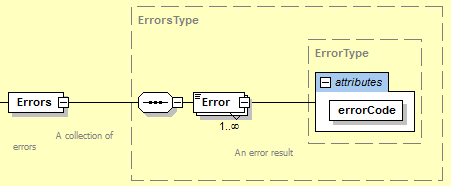
\includegraphics[width=1.0\textwidth]{figures/errors-schema-diagram.png}
  \caption{Errors Schema Diagram}
  \label{fig:errors-schema-diagram}
\end{figure}

\FloatBarrier

\tabulinesep = 5pt
\begin{longtabu} to \textwidth {
    |l|X[3l]|X[0.75l]|}
\caption{MTConnect Errors Element} \label{table:mtconnect-errors-element} \\

\hline
Element & Description & Occurrence \\
\hline
\endfirsthead

\hline
\multicolumn{3}{|c|}{Continuation of Table \ref{table:mtconnect-errors-element}}\\
\hline
Element & Description & Occurrence \\
\hline
\endhead
 
\gls{errors}	
&
An \gls{xml} container element in an \gls{mtconnecterrors response document} provided by an \gls{agent} when an error is encountered associated with a \gls{request} for information from a client software application.
\newline There \MUST be only one \gls{errors} element in an \gls{mtconnecterrors response document}.
\newline The \gls{errors} element \MUST contain at least one \gls{error} \gls{data entity} element.
&
1 \\
\hline


\end{longtabu}

\begin{note}
Note:	When compatibility with Version 1.0.1 and earlier of the MTConnect Standard is required for an implementation, the \gls{mtconnecterrors response document} contains only a single \gls{error} \gls{data entity} and the \gls{errors} \gls{structural element} \MUSTNOT appear in the document. 

\end{note}

\clearpage

\subsubsection{Error Data Entity}

When an \gls{agent} encounters an error when responding to a \gls{request} for information from a client software application, the information describing the error(s) is reported as a \gls{data entity} in an \gls{mtconnecterrors response document}.   \glspl{data entity} are organized in the \gls{errors} \gls{xml} container.

There is only one type of \gls{data entity} defined for an \gls{mtconnecterrors response document}.  That \gls{data entity} is called \gls{error}.

The following is an illustration of the structure of an \gls{xml} document demonstrating how \gls{error} \glspl{data entity} are reported in an \gls{mtconnecterrors response document}:

\begin{lstlisting}[firstnumber=1,escapechar=|,%
caption={Example of Error in MTConnectError}, label={lst:error-in mtconnecterror}]
<MTConnectError}>
  <Header/>
  <Errors>
    <Error/>
    <Error/>
    <Error/>
  </Errors>
</MTConnectError}>    
\end{lstlisting}

The \gls{errors} element \MUST contain at least one \gls{data entity}.  Each \gls{data entity} describes the details for a specific error reported by an \gls{agent} and is represented by the \gls{xml} element named \gls{error}.

\gls{error} \gls{xml} elements \MAY contain both attributes and \gls{cdata} that provide details further defining a specific error.  The \gls{cdata} \MAY provide the complete text provided by an \gls{agent} for the specific error.  

\paragraph{XML Schema Structure for Error}\mbox{}

The \gls{xml schema} in \fig{error-schema-diagram} represents the structure of an \gls{error} \gls{xml} element showing the attributes defined for \gls{error}.

\begin{figure}[ht]
  \centering
  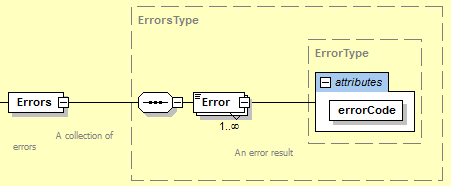
\includegraphics[width=0.75\textwidth]{figures/error-schema-diagram.png}
  \caption{Error Schema Diagram}
  \label{fig:error-schema-diagram}
\end{figure}

\FloatBarrier

\paragraph{Attributes for Error}\mbox{}

\gls{error} has one attribute.  \tbl{attributes-for-error} defines this attribute that provides additional information for an \gls{error} \gls{xml} element.   

\tabulinesep = 5pt
\begin{longtabu} to \textwidth {
    |l|X[3l]|X[0.75l]|}
\caption{Attributes for Error} \label{table:attributes-for-error} \\

\hline
Attribute & Description & Occurrence \\
\hline
\endfirsthead

\hline
\multicolumn{3}{|c|}{Continuation of Table \ref{table:attributes-for-error}}\\
\hline
Attribute & Description & Occurrence \\
\hline
\endhead
 
\gls{errorcode}
&
Provides a descriptive code that indicates the type of error that was encountered by an \gls{agent} when attempting to respond to a \gls{request} for information.
\newline \gls{errorcode} is a required attribute.
&
1 \\
\hline


\end{longtabu}

\paragraph{Values for errorCode}\mbox{}

There is a limited vocabulary defined for \gls{errorcode}.  The value returned for \gls{errorcode} \MUST be one of the following:

\newpage

\tabulinesep = 5pt
\begin{longtabu} to \textwidth {
    |l|X[3l]|}
\caption{Values for errorCode} \label{table:values-for-errorcode} \\

\hline
Value for errorCode & Description \\
\hline
\endfirsthead

\hline
\multicolumn{2}{|c|}{Continuation of Table \ref{table:values-for-errorcode}}\\
\hline
Value for errorCode & Description \\
\hline
\endhead

\gls{assetnotfound value}
&
The \gls{request} for information specifies an \gls{mtconnect asset} that is not recognized by the \gls{agent}.
\\ \hline

\gls{internalerror value}
&
The \gls{agent} experienced an error while attempting to published the requested information. 
\\ \hline


\gls{invalidrequest value}
&
The \gls{request} contains information that was not recognized by the \gls{agent}.
\\ \hline

\gls{invaliduri value}
&
The URI provided was incorrect. 
\\ \hline

\gls{invalidxpath value}
&
The \gls{xpath} identified in the \gls{request} for information could not be parsed correctly by the \gls{agent}.  This could be caused by an invalid syntax or the \gls{xpath} did not match a valid identify for any information stored in the \gls{agent}. 
\\ \hline

\gls{nodevice value}
&
The identity of the piece of equipment specified in the \gls{request} for information is not associated with the \gls{agent}.
\\ \hline

\gls{outofrange value}
&
The \gls{request} for information specifies \gls{streaming data} that includes sequence number(s) for pieces of data that are beyond the end of the \gls{buffer}.
\\ \hline

\gls{queryerror value}
&
The \gls{agent} was unable to interpret the \gls{query}.  The \gls{query} parameters do not contain valid values or include an invalid parameter.
\\ \hline

\gls{toomany value}
&
The \gls{count model} parameter provided in the \gls{request} for information requires either of the following:
\newline \tab- \gls{streaming data} that includes more pieces of data than the \gls{agent} is capable of organizing in an \gls{mtconnectstreams response document}. 
\newline \tab- Assets that include more \glspl{asset document} in an \gls{mtconnectassets response document} than the \gls{agent} is capable of handling. 
\\ \hline

\gls{unauthorized value}
&
The \gls{requester} does not have sufficient permissions to access the requested information.
\\ \hline

\gls{unsupported value}
&
A valid \gls{request} was provided, but the \gls{agent} does not support the feature or type of \gls{request}.
\\ \hline

\end{longtabu}

\paragraph{CDATA for Error}\mbox{}

The \gls{cdata} for \gls{error} contains a textual description of the error and any additional information an \gls{agent} is capable of providing regarding a specific error.  The \gls{valid data value} returned for \gls{error} \MAY be any text string.

\subsubsection{Examples for MTConnectError}

\lst{structure-for-mtconnecterror} is an example demonstrating the structure of an \gls{mtconnecterrors response document}:

\begin{lstlisting}[firstnumber=1,escapechar=|,% 
caption={Example of structure for MTConnectError}, label={lst:structure-for-mtconnecterror}]
<?xml version="1.0" encoding="UTF-8"?>
  <MTConnectError
  xmlns="urn:mtconnect.org:MTConnectError:1.4"
  xmlns:xsi=http://www.w3.org/2001/XMLSchema-instance
  xsi:schemaLocation="urn:mtconnect.org:MTConnectError
    :1.4/schemas/MTConnectError_1.4.xsd">
  <Header creationTime="2010-03-12T12:33:01Z"
    sender="MyAgent" version="1.4.1.10" 
    bufferSize="131000" instanceId="1383839" />
  <Errors>
    <Error errorCode="OUT_OF_RANGE" >Argument was 
      out of range</Error>
    <Error errorCode="INVALID_XPATH" >Bad 
      path</Error>
  </Errors>
</MTConnectError>
\end{lstlisting}

\lst{structure-for-mtconnecterror-when-backward-compatibility-is-required} is an example demonstrating the structure of an \gls{mtconnecterrors response document} when backward compatibility with Version 1.0.1 and earlier of the MTConnect Standard is required.  In this case, the \gls{document body} contains only a single \gls{error} \gls{data entity} and the \gls{errors} \gls{structural element} \MUSTNOT appear in the document. 

\begin{lstlisting}[firstnumber=1,escapechar=|,% 
caption={Example of structure for MTConnectError when backward compatibility is required}, label={lst:structure-for-mtconnecterror-when-backward-compatibility-is-required}]
<?xml version="1.0" encoding="UTF-8"?>
<MTConnectError
  xmlns="urn:mtconnect.org:MTConnectError:1.1"
  xmlns:xsi=http://www.w3.org/2001/XMLSchema-instance
  xsi:schemaLocation="urn:mtconnect.org:MTConnectError
    :1.1/schemas/MTConnectError_1.1.xsd">
  <Header creationTime="2010-03-12T12:33:01Z"
    sender="MyAgent" version="1.1.0.10" 
    bufferSize="131000" instanceId="1383839" />
  <Error errorCode="OUT_OF_RANGE" >Argument was out 
    of range</Error>
</MTConnectError>
\end{lstlisting}

